% ----------------------------------------------------------
% Ajuda.Ai
% ----------------------------------------------------------
\chapter{Ajuda.Ai} \label{cha:ajudaai}

O projeto Ajuda.Ai é um software de código-fonte aberto que visa ajudar instituições a arrecadar doações através da internet e aos usuários a doarem para instituições de forma simples, semelhante a adquirir um produto numa loja online, ter uma boa integração junto a plataformas de redes sociais e unir doadores e instituições. O projeto apresentado foi construído com uma interface para ser acessada pelo navegador através de uma aplicação web de página única (\emph{Single Page Application}), além de contar com uma API que dá suporte a outros tipos de interface, e no lado do servidor uma aplicação Java em um servidor de aplicação RedHat WildFly 10.

O código-fonte da ferramenta está disponível sob licença MIT no endereço \\ https://github.com/g0dkar/ajuda-ai e está publicada no endereço https://ajuda.ai. A API pode ser acessada através do \emph{endpoint} https://api.ajuda.ai/v1. Apesar da ferramenta estar pronta para uso, por hora nenhuma instituição real está sendo contemplada, mas duas instituições reais encontram-se cadastradas apenas para testes. Elas serão as primeiras a serem contactadas para iniciarem o uso do Ajuda.Ai. A divulgação da ferramenta será feita inicialmente através de contato direto com as Instituições e através de redes sociais. Futuramente, publicidades digitais podem ser uma opção viável para ajudar a trazer mais doadores e novas instituições ao Ajuda.Ai.





\section{Casos de Uso} \label{sec:ajudaai:casos}

O levantamento de requisitos foi feito através da análise do mercado de \emph{crowdfunding} nacional, do crescimento e popularização da prática dessa modalidade de investimento, tendencias internacionais em relação ao mercado de empreendimentos sociais e leitura e análise da literatura exposta no capítulo \ref{cha:fundamentacao}. Os casos de uso relevantes resultantes do levantamento de requisitos foram:

\begin{lista}
  \item \textbf{Caso de Uso 01 - Doação}: O usuário se identifica com o trabalho de uma determinada instituição e quer fazer uma doação a mesma através da Internet;
  \item \textbf{Caso de Uso 02 - Comunicação com o Doador}: As instituições precisam de um canal para se comunicarem aos seus doadores e potenciais doadores;
  \item \textbf{Caso de Uso 03 - Acompanhamento das Doações}: É importante para a Instituição ter uma maneira de acompanhar a arrecadação de sua campanha e ter informações sobre quanto foi arrecadado e quando o dinheiro estará disponível;
  %\item \textbf{Caso de Uso 04 - Descobrimento de Instituições}: É importante para a Instituição ter uma maneira de acompanhar a arrecadação de sua campanha e ter informações sobre quanto foi arrecadado e quando o dinheiro estará disponível;
\end{lista}

As especificações dos casos de uso estão disponíveis no Anexo \ref{anexo:b} - Especificação de Casos de Uso. Apesar de outros casos de uso existirem, por serem bastante simples e triviais, como \emph{login}, \emph{logout}, CRUD simples de entidades do projeto \codigo{model} (apresentado no item \ref{sec:ajudaai:organizacao}) eles não foram documentados. Esses casos de uso são inclusos no diagrama de Casos de Uso, ilustrado na Figura \ref{fig:uml_caso_uso}.

\begin{figure}[H]
  \caption{\label{fig:uml_caso_uso}Diagrama UML de Casos de Uso do Ajuda.Ai}
  \centering
  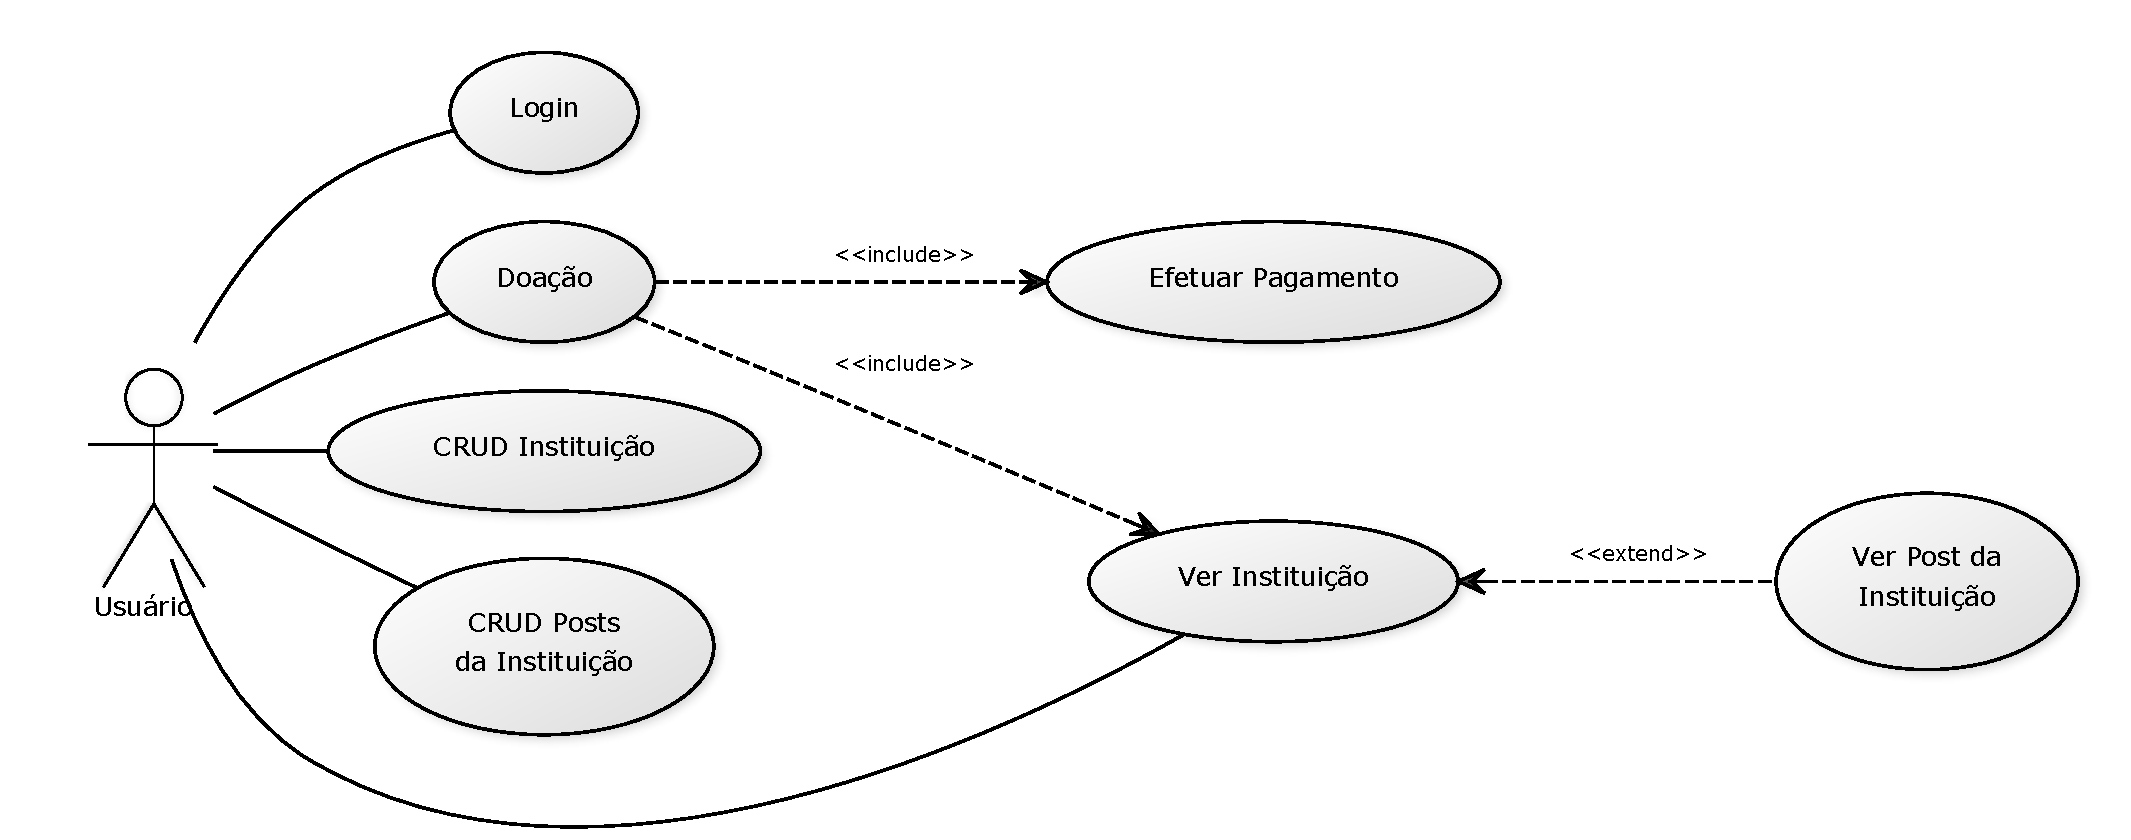
\includegraphics[scale=0.4]{imagens/uml-casos-de-uso-02.pdf}
  \legend{Fonte: Elaborado pelo Autor}
\end{figure}

A seguir serão apresentados detalhes sobre a implementação do projeto, como tecnologias utilizadas, e em seguida uma apresentação visual da aplicação criada. Por fim, uma parte mais detalhada sobre partes importantes do sistema e sua API REST Web.





\section{Características da Implementação} \label{sec:ajudaai:caracteristicas}

O sistema utiliza a plataforma Java em sua versão 8. Para facilitar a configuração da aplicação e gestão de dependências se utilizou a ferramenta Apache Maven\footnote{https://maven.apache.org}, que provê um fácil acesso a uma grande quantidade de ferramentas e bibliotecas. Além da resolução de dependências, o Apache Maven facilita o processo de construção e montagem da aplicação, automatiza a produção da documentação da aplicação apartir do JavaDoc\footnote{Padrão de documentação Java que utiliza comentários com formatação para documentar a aplicação} e é considerado uma ferramenta padrão da indústria.

Como arcabouço para desenvolvimento de aplicação web se utilizou o Caelum VRaptor. O VRaptor é um arcabouço brasileiro MVC de código fonte aberto que traz alta produtividade para um desenvolvimento Java Web rápido e fácil com CDI\footnote{Retirado de http://www.vraptor.org/pt/ em 17/02/2017}. Dentre as funcionalidades mais interessantes do VRaptor estão a integração completa e simples com o arcabouço JBoss Weld, implementação de referência da especificação JSR 365\footnote{Especificação Java para um sistema de Injeção de Dependências usando o Padrão de Projeto Inversão de Controle} e arcabouço utilizado pelo RedHat Wildfly 10, e o uso do estilo convenção sob configuração onde se promove que, seguindo convenções bem definidas, não é necessário arquivos de configuração.

Para persistência de dados foi utilizado o arcabouço JBoss Hibernate ORM. Como um arcabouço de mapeamento objeto-relacional o Hibernate ORM faz a persistência de dados em banco de dados relacionais via JDBC\footnote{Retirado de http://hibernate.org/orm/ em 17/02/2017}. Como solução para banco de dados foi utilizado o SGBD MariaDB, banco de dados de código aberto que surgiu a partir do MySQL quando o mesmo foi comprado pela Oracle em 2003. Ele é mantido pelos desenvolvedores originais do MySQL e eles garantem que sempre será um projeto de código aberto. usuários notáveis incluem Wikipedia, WordPress.com e Google\footnote{Retirado de https://mariadb.org/about/ em 17/02/2017}.

Por fim, senhas são criptografadas no banco de dados se utilizando do algoritmo BCrypt. O BCrypt é uma função de \emph{hashing} de senhas projetada em 1999 por Niels Provos e David Mazières baseada na cifra \emph{Blowfish} que também incorporara um \emph{salt}\footnote{Bytes gerados de forma aleatória} para proteger as senhas contra ataques de tabelas arco-íris\footnote{\emph{Rainbow Table Attack}: Ataque que consiste em gerar um gigantesco banco de dados de \emph{hashes} pré-processados onde é possível se buscar pelo texto simples de um determinado \emph{hash} de um determinado algoritmo}. Nesse contexto, a maior vantagem do BCrypt é que esta é uma função cuja a quantidade de iterações pode ser configurada e assim, com o tempo, pode ser aumentada para torná-la mais lenta e resistente a ataques de força-bruta \cite{wiki:Bcrypt}.





\section{Apresentação da Aplicação} \label{sec:ajudaai:apresentacao}
%\textbf{\textit{Aqui será apresentado screenshots e essas coisas. Ainda não sei exatamente de que maneira ou que texto escrever para apresentar as figuras. Talvez um run-down do processo de doação?}}

Nesta seção será apresentada de forma ilustrada a solução desenvolvida neste trabalho. Parte do projeto visual, cores e detalhes estéticos são de autoria de Cândido Sales Gomes. A Figura \ref{fig:ss_ajudaai_01} apresenta a página inicial do projeto Ajuda.Ai. Nela temos um painel rotativo informativo com âncoras para páginas informativas sobre o projeto, uma lista mesclada entre instituições mais recentemente cadastradas no projeto e outras escolhidas aleatoriamente e uma seção com um pequeno mapa de âncoras para todas as páginas informativas do projeto.

\begin{figure}[H]
	\caption{\label{fig:ss_ajudaai_01}Captura de Tela da Página Inicial do Projeto Ajuda.Ai}
    \centering
    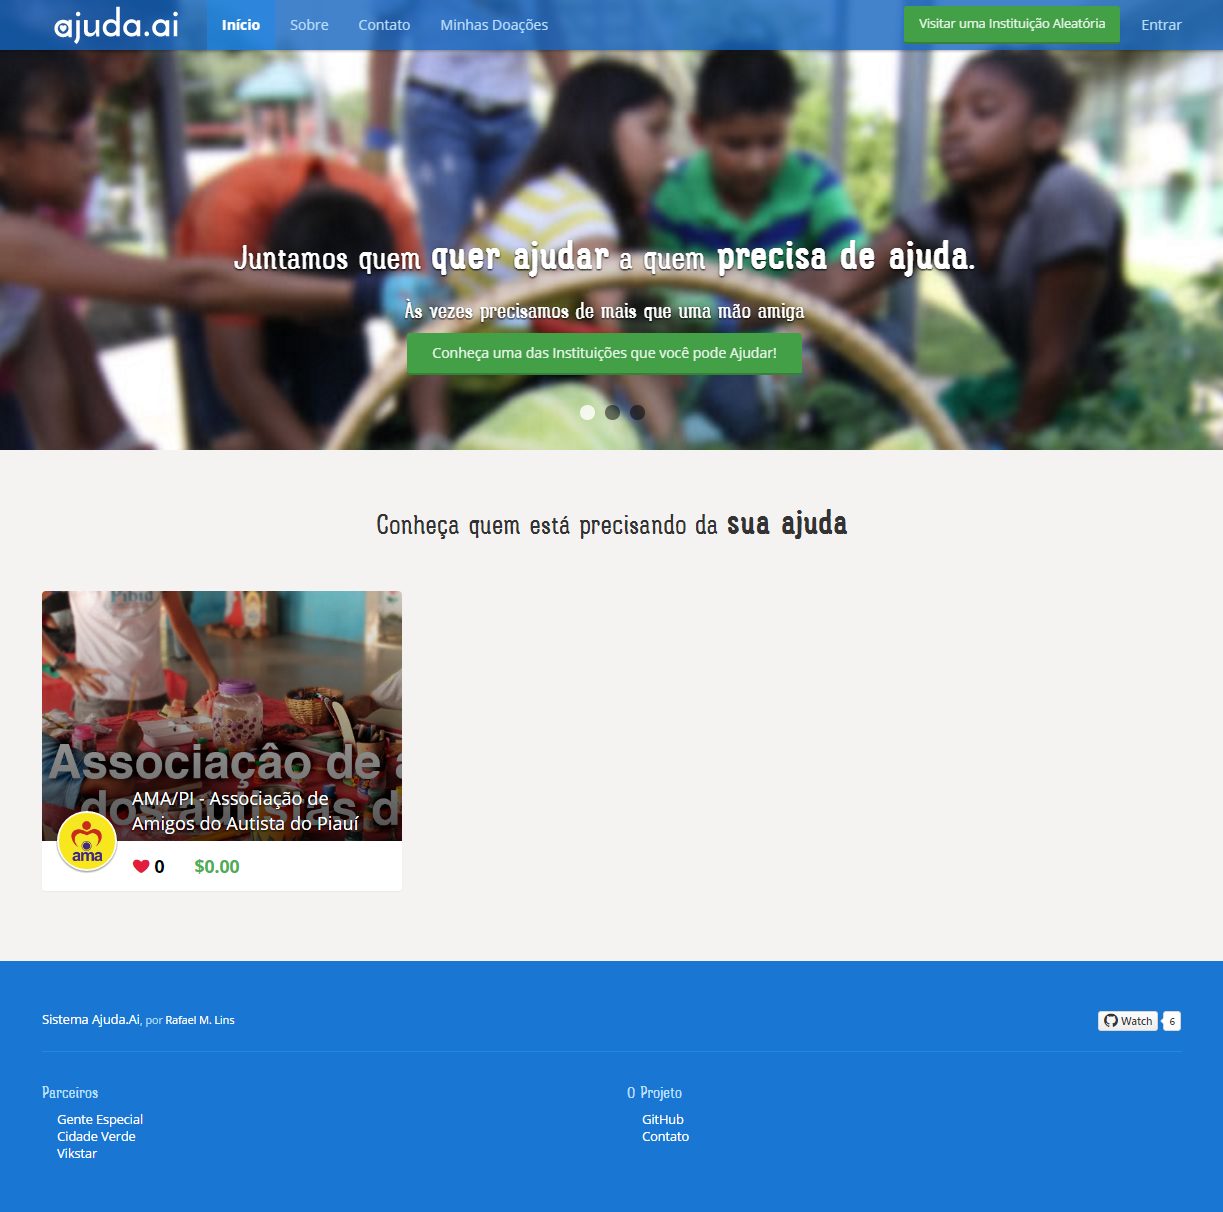
\includegraphics[scale=0.45]{imagens/screenshot-ajudaai-01.png}
    \legend{Fonte: Elaborado pelo Autor}
\end{figure}

A estrutura das páginas segue em grande parte a mesma estrutura visual na Figura \ref{fig:ss_ajudaai_01}: uma barra de navegação de posicionamento fixo no topo da tela, um painel com uma grande figura e uma frase de cabeçalho, o conteúdo da página atual e o rodapé.

Na Figura \ref{fig:ss_ajudaai_02} é apresentada uma página interna, especificamente a página ``Sobre'', que fala em linhas gerais sobre o projeto. Esse mesmo modelo é utilizado para todas as páginas internas, representadas pela entidade \codigo{Page}, apresentada na seção \ref{sec:ajudaai:organizacao}.

\begin{figure}[H]
	\caption{\label{fig:ss_ajudaai_02}Captura de Tela da Página Sobre do Projeto Ajuda.Ai}
    \centering
    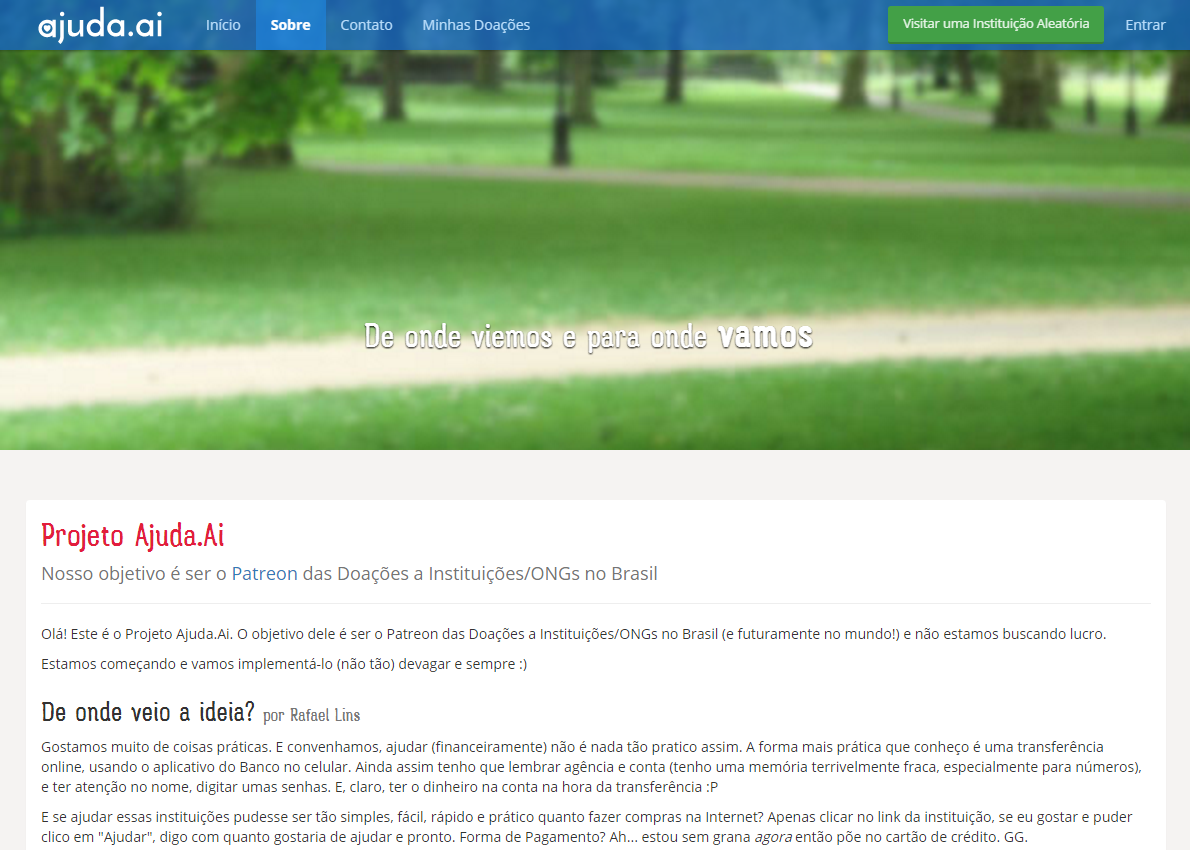
\includegraphics[scale=0.45]{imagens/screenshot-ajudaai-02.png}
    \legend{Fonte: Elaborado pelo Autor}
\end{figure}

A seguir, na Figura \ref{fig:ss_ajudaai_03} é apresentada uma página de Instituição. Elementos visuais como a imagem do painel e logomarca da instituição são personalizáveis através de configurações da interface de administração. Além disso, é apresentada ao navegante uma contagem atualizada de quantas doações a instituição recebeu e o valor total das doações. O projeto visual do Ajuda.Ai se utiliza uma técnica de comunicação chamada \emph{Call-To-Action} onde elementos que invocam ações, como botões, têm seu texto escrito de forma imperativa a fim de incentivar quem o lê a tomar a ação. É possível observar um uso da técnica no botão ``Quero Ajudar'' na Figura \ref{fig:ss_ajudaai_03}, o qual leva o usuário a página onde é possível se fazer uma doação.

\begin{figure}[H]
	\caption{\label{fig:ss_ajudaai_03}Captura de Tela da Página da Instituição AMA do Projeto Ajuda.Ai}
    \centering
    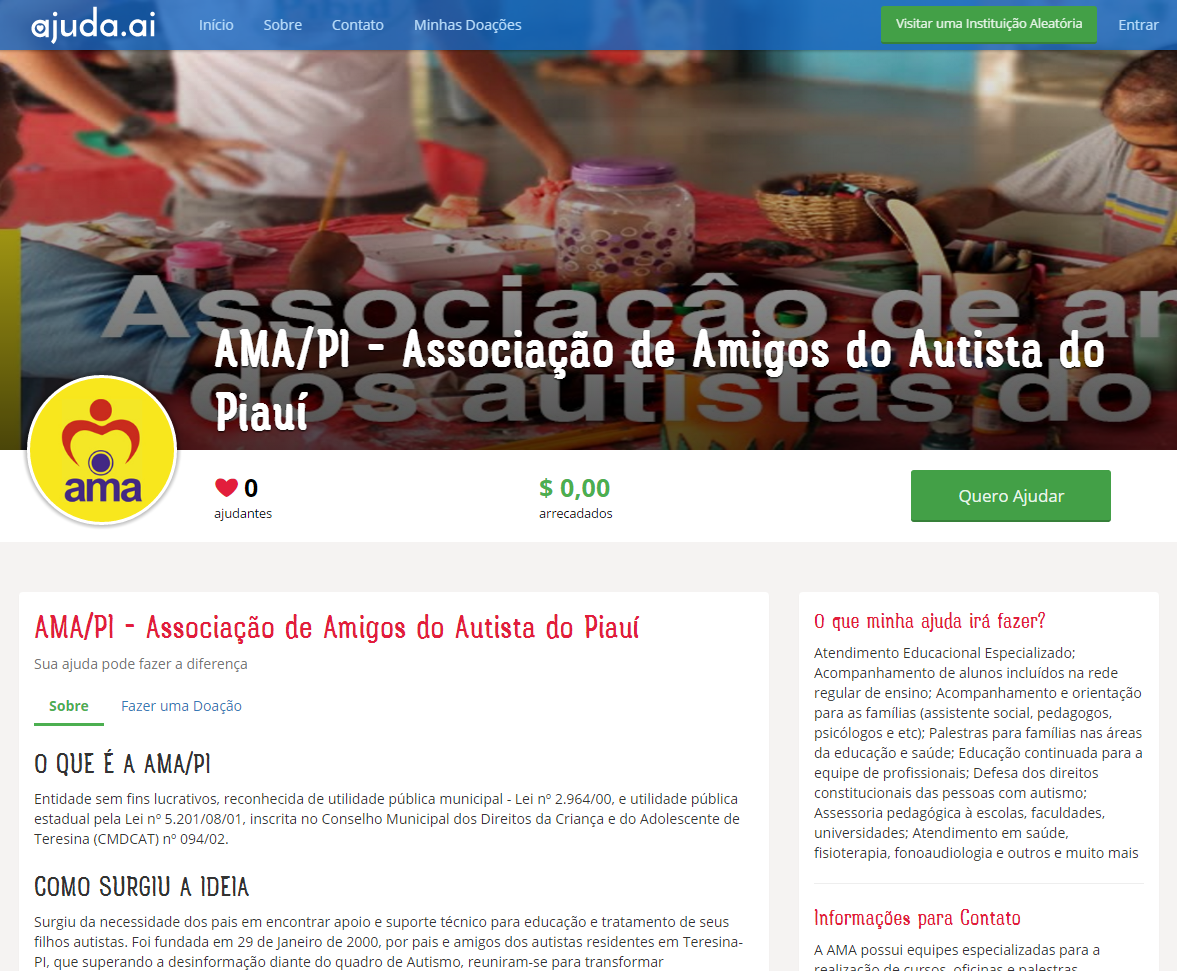
\includegraphics[scale=0.45]{imagens/screenshot-ajudaai-03.png}
    \legend{Fonte: Elaborado pelo Autor}
\end{figure}

Ao clicar no botão ``Quero Ajudar'' ou na aba ``Fazer uma Doação'', o usuário é levado a página de doação, cujo conteúdo é exibido na Figura \ref{fig:ss_ajudaai_04}. Como forma de incentivo a doações maiores, uma singela forma de \emph{gamefication}\footnote{Técnica onde se introduz elementos de jogos a fim de otimizar a execução de certas ações} foi utilizada na forma de uma barra de progresso com marcadores que é preenchida de acordo com o valor da doação, inicialmente em R\$ 20,00. É dada a opção de anonimato através da proibição da exibição do nome do doador. O nome e e-mail serão gravados para a emissão da ordem de pagamento junto ao \emph{Gateway}, mas se a publicação for proibida o nome não será exibido em lugar algum, nem mesmo para a instituição que recebeu a doação.

Por segurança, a página também inclui um teste CAPTCHA do serviço Google reCAPTCHA. O serviço reCAPTCHA é um sistema de caixa de diálogo para usuário baseado na interface do CAPTCHA, que pede para usuários digitarem palavras distorcidas exibidas na tela, para ajudar a digitalizar o texto de livros, enquanto protege \emph{sites} de robôs tentando acessar áreas restritas. O serviço fornece, para os \emph{sites} inscritos, imagens de palavras que o software de reconhecimento ótico de caracteres (OCR) não foi capaz de identificar as quais são apresentadas para humanos decifrarem como palavras CAPTCHAs, como parte do seu procedimento normal de validação. Depois eles retornam os resultados para o serviço reCAPTCHA, que envia esses resultados para a digitalização de seus projetos \cite{wiki:ReCAPTCHA}.

\begin{figure}[H]
	\caption{\label{fig:ss_ajudaai_04}Captura de Tela do Formulário de Doação}
    \centering
    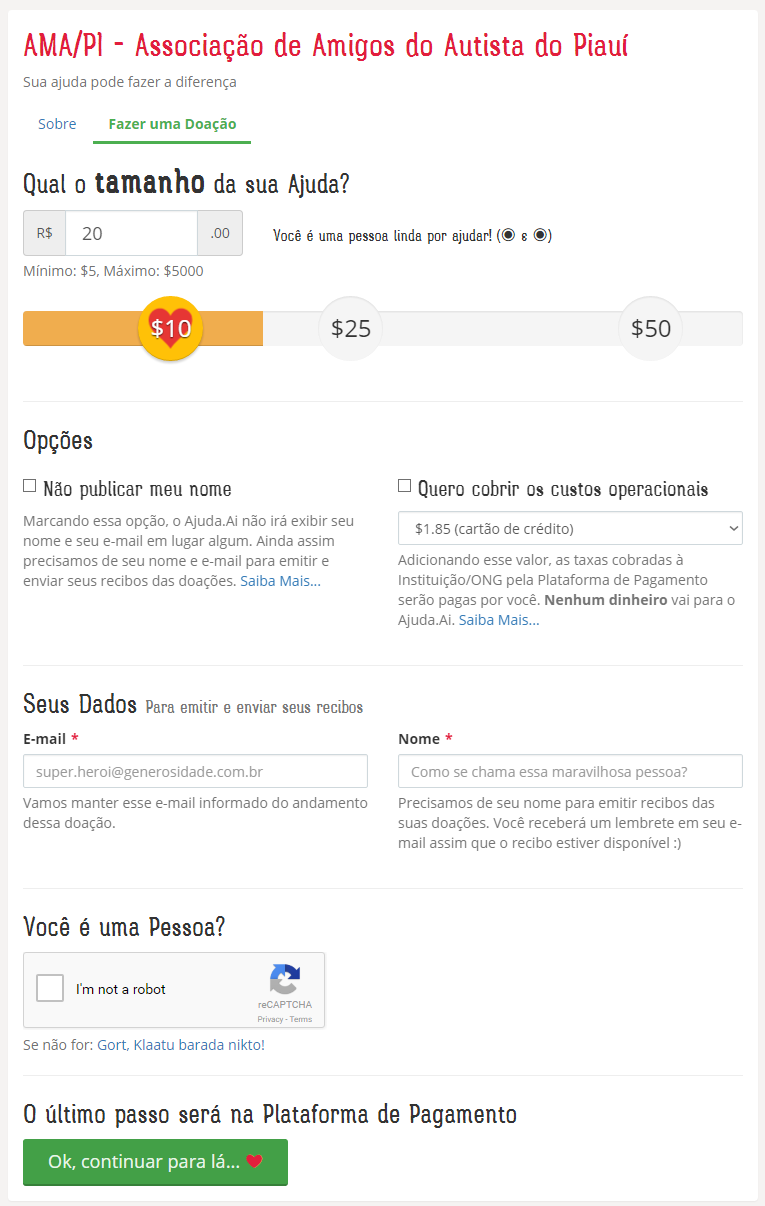
\includegraphics[scale=0.5]{imagens/screenshot-ajudaai-04.png}
    \legend{Fonte: Elaborado pelo Autor}
\end{figure}

Essa interface com o usuário através de uma folha de estilos CSS adequada pode se adaptar ao dispositivo onde a página está sendo exibida. Nas Figuras \ref{fig:ss_ajudaai_05} e \ref{fig:ss_ajudaai_06} temos duas capturas de tela mostrando como a interface se adapta quando exibida em um telefone celular.

\begin{figure}[H]
 \centering
  \begin{minipage}{0.4\textwidth}
    \centering
    \caption{Captura de Tela da Página Inicial em Dispositivo Móvel}
    \label{fig:ss_ajudaai_05}
    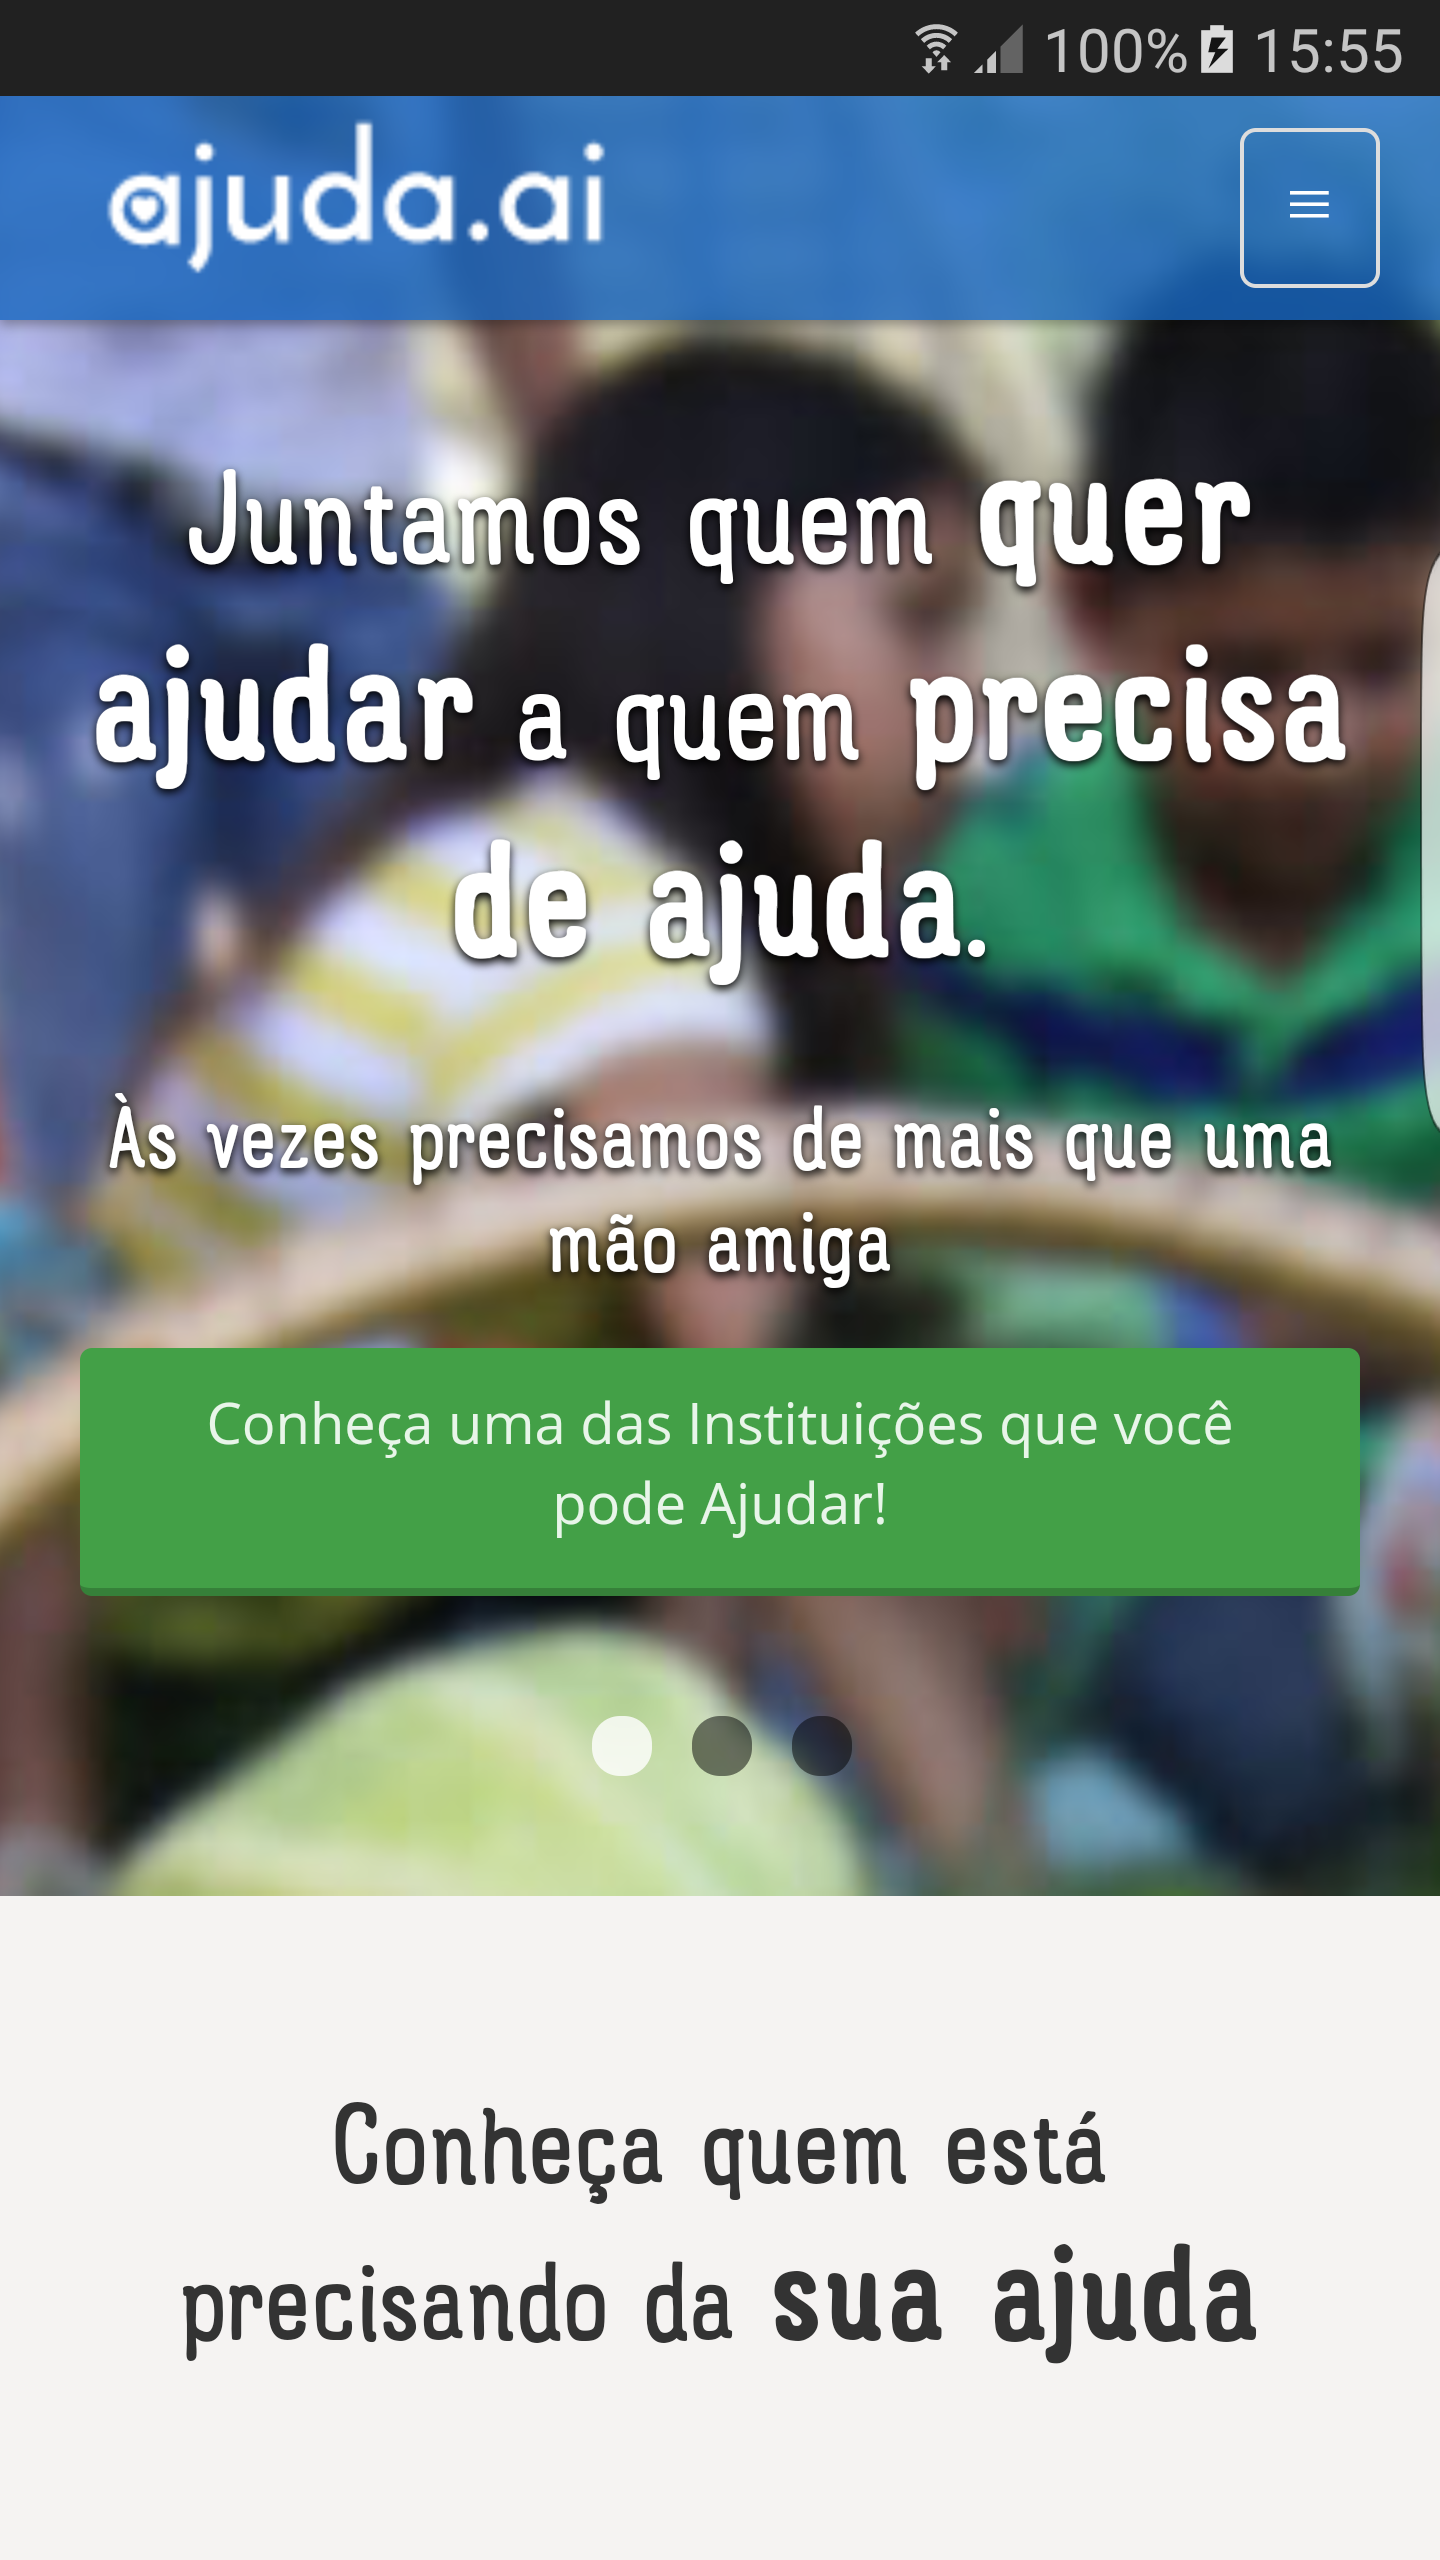
\includegraphics[scale=0.12]{imagens/screenshot-ajudaai-05.png}
    \legend{Fonte: Elaborado pelo Autor}
  \end{minipage}
  \hfill
  \begin{minipage}{0.4\textwidth}
    \centering
    \caption{Captura de Tela de Página de Instituição em Dispositivo Móvel}
    \label{fig:ss_ajudaai_06}
    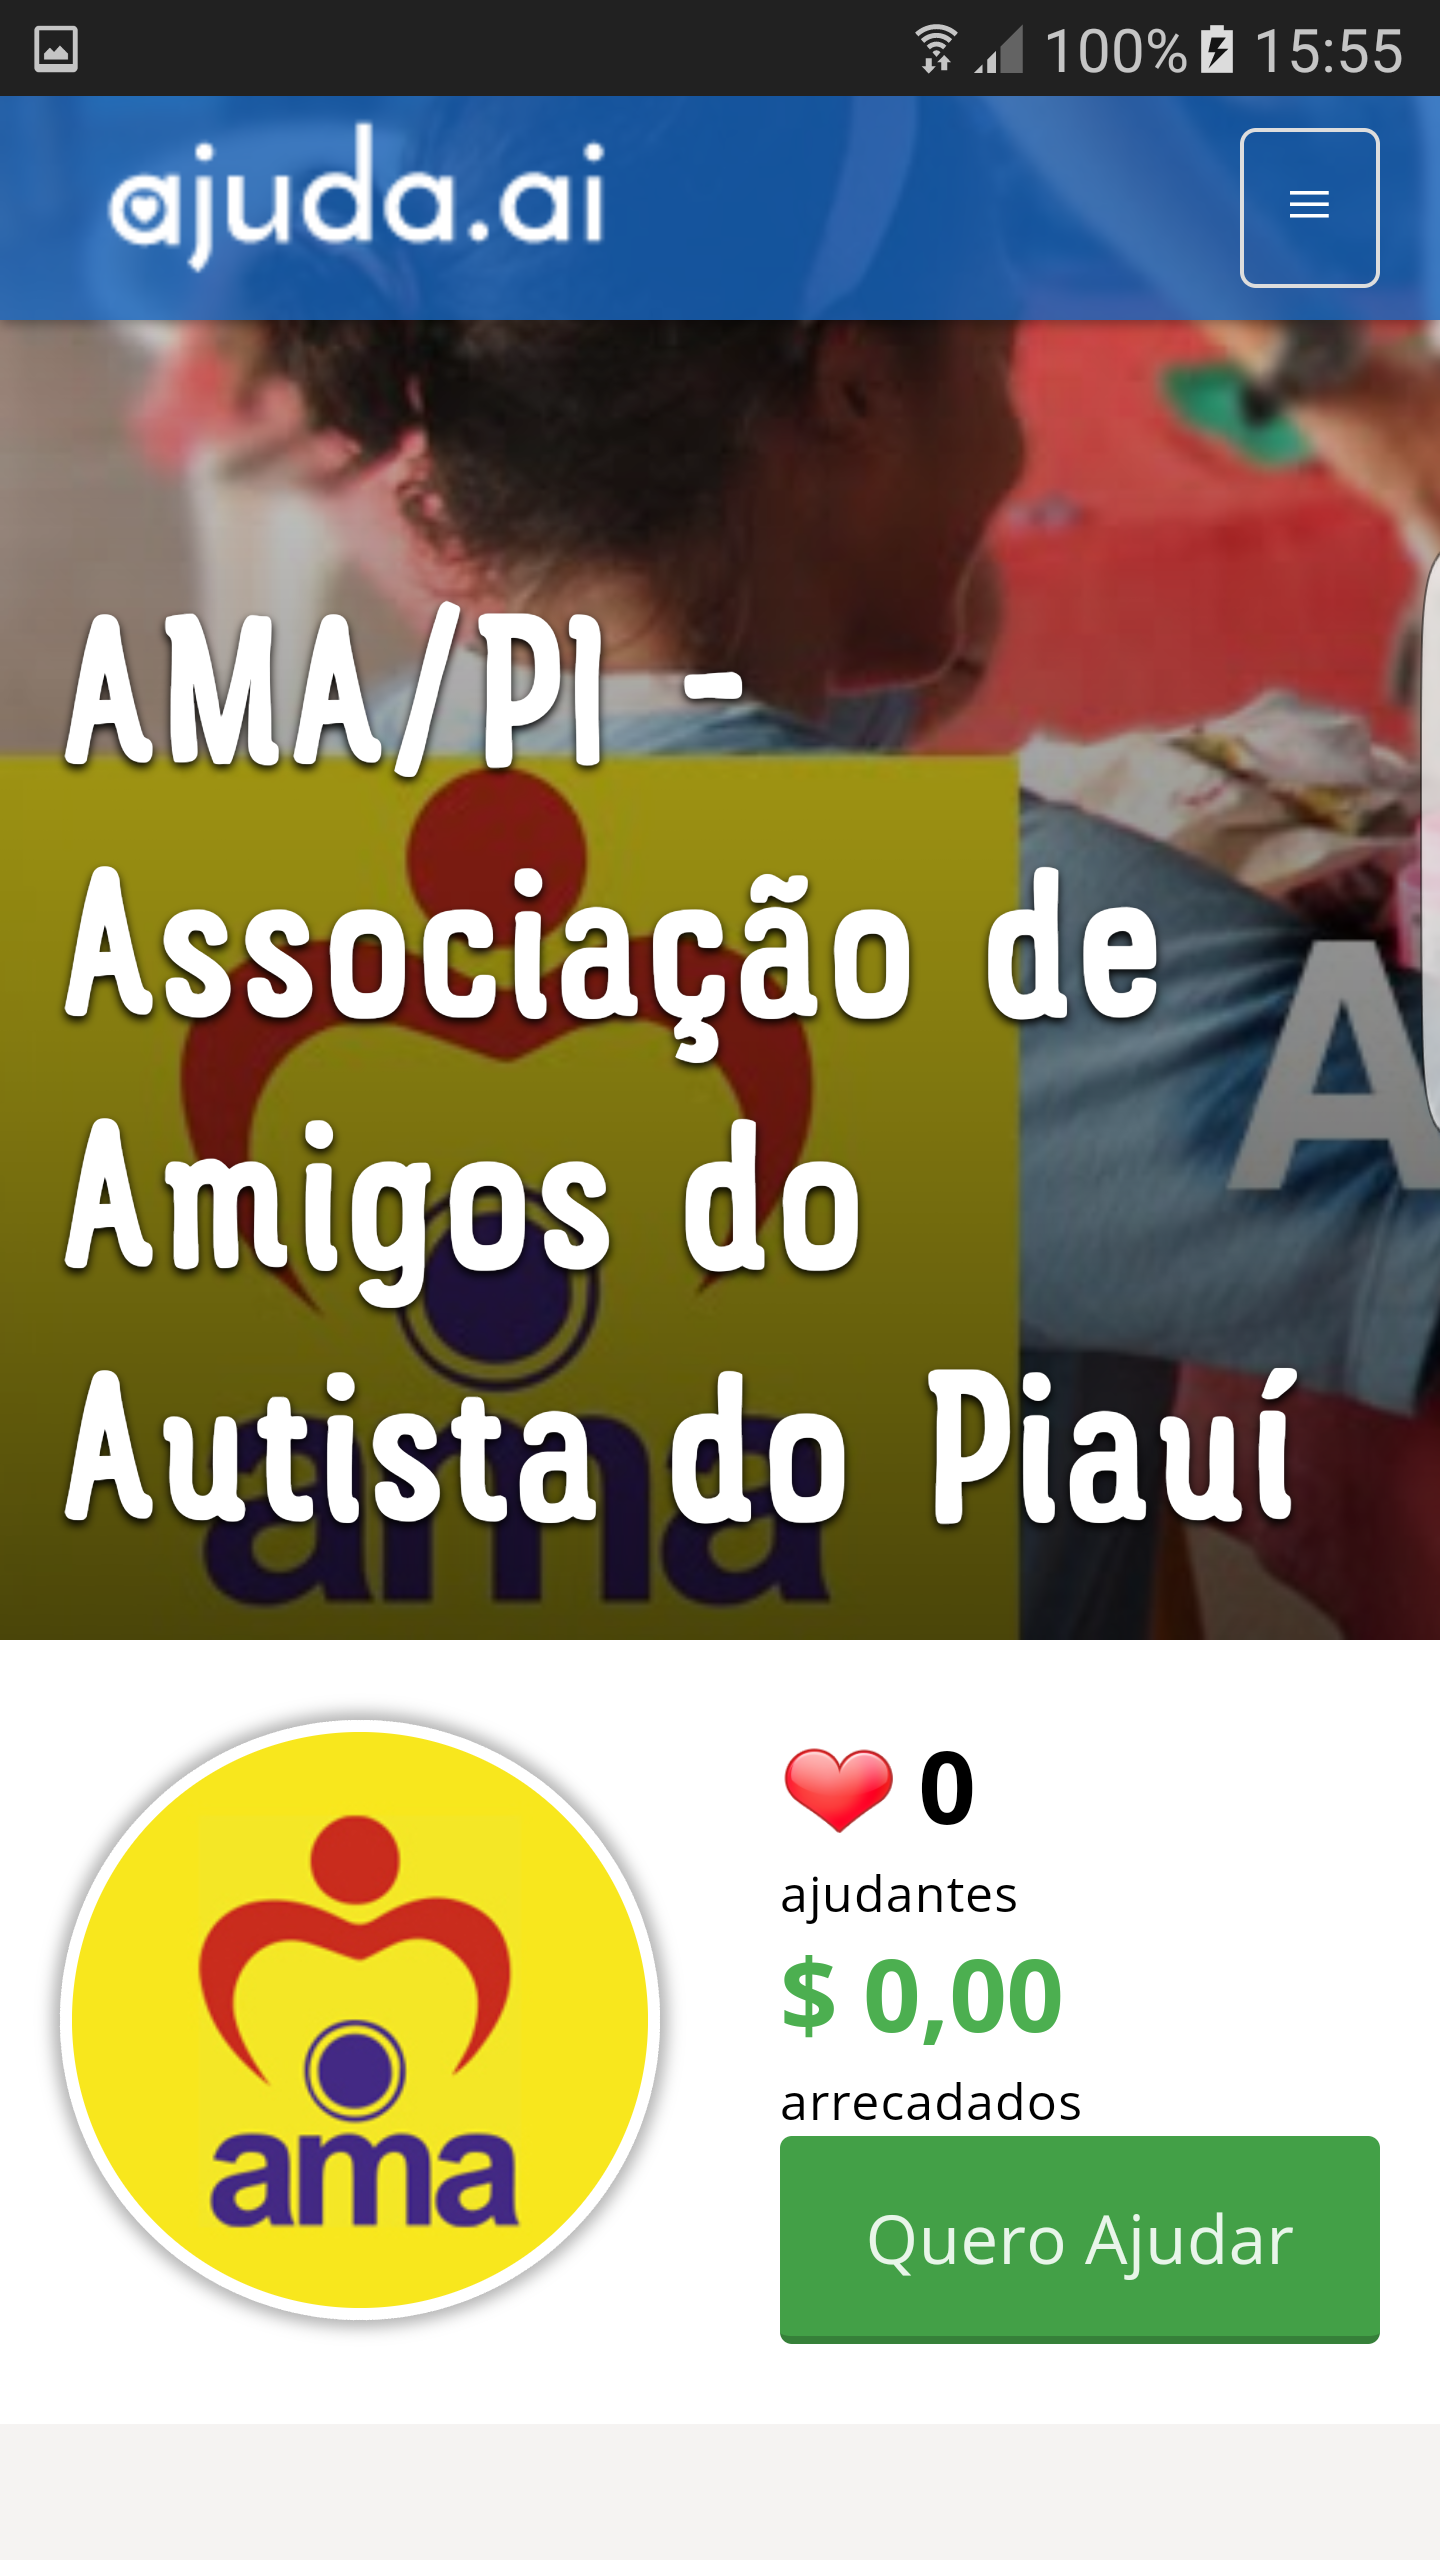
\includegraphics[scale=0.12]{imagens/screenshot-ajudaai-06.png}
    \legend{Fonte: Elaborado pelo Autor}
  \end{minipage}
\end{figure}

Essa capacidade é uma das melhores práticas recomendadas pela indústria, pois melhora a gama de usuários que terão acesso adequado à página. Esse aspecto é importante para o Ajuda.Ai devido a sua proposta de ser um meio de acesso a uma grande comunidade de pessoas, através de redes sociais, e ao crescimento da quantidade de dispositivos móveis no Brasil e do acesso a Internet através destes dispositivos.

Na Figura \ref{fig:ss_ajudaai_07} temos a tela de Login do usuário. O acesso a área administrativa pode ser feito através do nome de usuário escolhido ao se registrar ou e-mail. As senhas, como explicado na seção \ref{sec:ajudaai:caracteristicas}, são criptografadas com BCrypt e, como consequência, são conhecidas apenas pelos seus donos. Na mesma tela, caso o usuário tenha esquecido sua senha, é possível se utilizar o link ``Esqueci minha senha'' para que, usando o nome de usuário ou e-mail preenchido, um e-mail com instruções para reinicialização de senha será enviado para o usuário, a partir do qual ele poderá criar uma nova senha.

\begin{figure}[H]
	\caption{\label{fig:ss_ajudaai_07}Captura de Tela de Login do Ajuda.Ai}
    \centering
    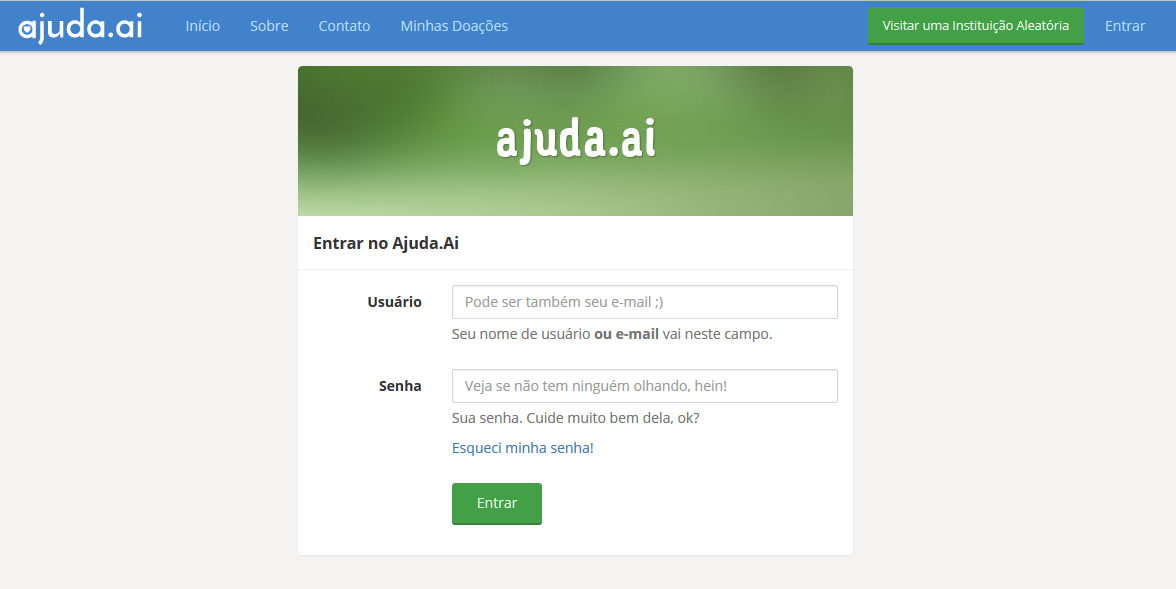
\includegraphics[scale=0.48]{imagens/screenshot-ajudaai-07.png}
    \legend{Fonte: Elaborado pelo Autor}
\end{figure}

Após o \emph{login}, na Figura \ref{fig:ss_ajudaai_08}, um \emph{dashboard} com informações relevantes são mostradas ao usuário: Suas últimas doações, total doado, quantidade de instituições ajudadas, média do valor das doações, últimas notícias das instituições ajudadas e quais as últimas doações feitas. Essa tela é também o que é exibido quando o usuário utiliza o link ``Minhas Doações'' do menu principal.

\begin{figure}[H]
	\caption{\label{fig:ss_ajudaai_08}Captura do \emph{Dashboard} de Doações, com dados de exemplo}
    \centering
    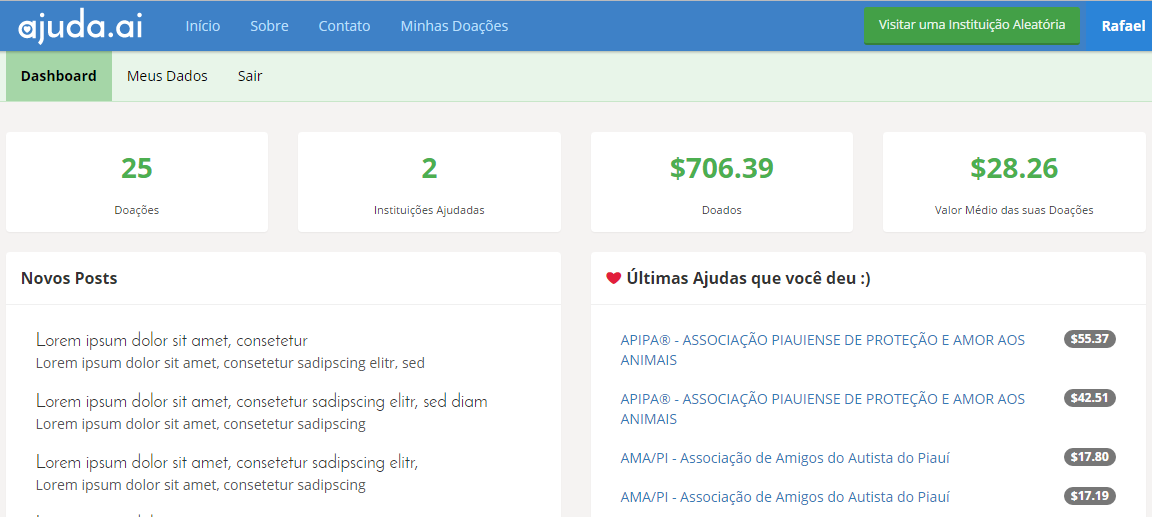
\includegraphics[scale=0.5]{imagens/screenshot-ajudaai-08.png}
    \legend{Fonte: Elaborado pelo Autor}
\end{figure}










\section{Organização do Projeto} \label{sec:ajudaai:organizacao}
O projeto está organizado numa estrutura de Projeto Pai e Projetos Filhos do Apache Maven. Essa organização facilita na manutenção e montagem da aplicação no momento da distribuição ou \emph{deployment} da mesma. Os projetos filhos são:

\begin{lista}
  \item \textbf{util}: Classes utilitárias usado pelos outros projetos. As duas classes mais utilizadas são \codigo{StringUtils}, com utilitários para comparação e processamento de Strings, e \codigo{SendMail}, que utiliza a API \codigo{javax.mail} para enviar e-mails como HTML;
  \item \textbf{model}: Contém o modelo de dados do Ajuda.Ai, apresentado na Figura \ref{fig:uml_model};
  \item \textbf{persistence-sql}: Provê classes que implementam a persistência do projeto model em um banco de dados SQL através do JBoss Hibernate;
  \item \textbf{backend}: Servidor de Back-end do Ajuda.Ai. Aplica as regras de negócio, organiza pagamentos e atende requisições dos usuários;
  \item \textbf{frontend}: Aplicação de Página Única do Front-end do Ajuda.Ai. Uma interface web simples e agradável para utilização do sistema;
  \item \textbf{payment-api}: Projeto pai para as implementações de pagamentos dos diferentes \emph{Gateways} de pagamento;
  \item \textbf{payment-impl-moip}: Implementação de payment-api para o \emph{gateway} MoIP;
  \item \textbf{payment-impl-pagseguro}: Implementação de payment-api para o \emph{gateway} PagSeguro;
  %\item \textbf{tests}: Testes do sistema.
\end{lista}

O modelo de dados da aplicação é apresentado na Figura \ref{fig:uml_model}, onde é apresentado um diagrama UML de classes do projeto \emph{model}. Estas são as principais entidades do sistema e seus relacionamentos:

\begin{lista}
%% ajuda.ai.model.user
\item \codigo{\textbf{User}}: Usuário simples. Todos os usuários podem ter Instituições e só poderão alterar informações vinculadas a ele mesmo;

%% ajuda.ai.model.extra
\item \codigo{\textbf{CreationInfo}}: Entidade embarcável\footnote{Uma Entidade Embarcável é uma classe que, no esquema objeto-relacional da plataforma Java, não tem uma tabela no SGBD própria e sim faz parte da tabela das classes que se associam a esta classe.} que guarda quando uma entidade foi criada, que usuário a criou, quando foi feita a última alteração na entidade e qual usuário fez a alteração. Caso o usuário que criou ou alterou seja nulo se considera que foi uma ação tomada pelo próprio Sistema;
\item \codigo{\textbf{Page}}: Uma página de conteúdo livre do Ajuda.Ai. Representa uma página web cujo conteúdo mude com pouca frequência;

%% ajuda.ai.model.institution
\item \codigo{\textbf{Institution}}: Representa uma Instituição criada por um Usuário;
\item \codigo{\textbf{InstitutionPost}}: Uma página de conteúdo livre vinculada a uma Instituição. Estende \codigo{Page};

%% ajuda.ai.model.billing
\item \codigo{\textbf{Payment}}: Representa uma ordem de pagamento feita pelo Sistema a um \emph{Gateway} de Pagamento em nome de um Usuário;
\item \codigo{\textbf{PaymentEvent}}: Representa uma mudança de estado de um pagamento como informado pelo \emph{Gateway} de Pagamento;
\end{lista}

%As principais classes do sistema são \codigo{Instituion}, \codigo{Payment} e \codigo{PaymentEvent}. A primeira representa as Instituições cadastradas no sistema, as quais receberão doações de usuários, representados por \codigo{User}. Essas doações são representadas internamente como objetos \codigo{Payment} os quais abstraem de forma unificada pagamentos feitos através de diferentes \emph{Gateways} de Pagamento. Por fim, o andamento do pagamento junto ao \emph{Gateway} é informado através de notificações, como explicado em \ref{sec:ajudaai:processo_pagamento}, e essas notificações são, então, abstraídas como objetos \codigo{PaymentEvent} vinculados a um \codigo{Payment}.

\begin{figure}[H]
	\caption{\label{fig:uml_model}Diagrama UML de Classes Resumido do Modelo do Ajuda.Ai}
    \centering
	\begin{tikzpicture}
    	\begin{umlpackage}[x=-3.5, y=0]{ajuda{.}ai{.}model{.}user}
        	\umlclass[x=0, y=0]{User}{
            	- id : Long \\
				- username : String \\
				- password : String \\
				- email : String \\
				- firstname : String \\
				- lastname : String
            }{}
		\end{umlpackage}
        
        \begin{umlpackage}[x=-1.5, y=-15]{ajuda{.}ai{.}model{.}billing}
        	\umlclass[x=0, y=0]{Payment}{
            	- id : Long \\
                - uuid : String \\
				- institution : Institution \\
                - creation : CreationInfo \\
				- description : String \\
				- paymentService : String \\
				- paymentServiceId : String \\
				- value : int \\
				- realValue : int \\
				- paid : boolean \\
				- readyForAccounting : boolean \\
				- cancelled : boolean \\
				- payeeName : String \\
				- payeeEmail : String \\
				- events : List<PaymentEvent>
            }{}
            \umlclass[x=7.5, y=0]{PaymentEvent}{
            	- id : Long \\
                - payment : Payment \\
				- timestamp : Date \\
				- transactionServiceId : String \\
				- status : int \\
				- currency : String \\
				- value : int \\
				- paymentType : String \\
				- paymentTypeInfo : String
            }{}
		\end{umlpackage}
        
        \begin{umlpackage}[x=2.7, y=0]{ajuda{.}ai{.}model{.}extra}
        	\umlclass[x=4.8, y=0]{Page}{
            	- id : Long \\
				- slug : String \\
				- creation : CreationInfo \\
				- headerImage : String \\
				- title : String \\
				- subtitle : String \\
				- content : String \\
				- published : boolean
            }{}
            \umlclass[x=0, y=0]{CreationInfo}{
            	- time : Date \\
				- lastUpdate : Date \\
				- creator : User \\
				- lastUpdateBy : User
            }{}
		\end{umlpackage}
        
        \begin{umlpackage}[x=-2.1, y=-6.5]{ajuda{.}ai{.}model{.}institution}
        	\umlclass[x=0, y=0]{Institution}{
            	- id : Long \\
				- slug : String \\
				- creation : CreationInfo \\
				- name : String \\
				- description : String \\
				- paymentService : String \\
				- attributes : Map<String, String>
            }{}
            \umlclass[x=6.5, y=0]{InstitutionPost}{
				- institution : Institution \\
				- pageviews : long
            }{}
		\end{umlpackage}
        
        
		
        
        
        \umlinherit[very thick]{InstitutionPost}{Page}
        \umlcompo[very thick]{CreationInfo}{User}
        \umlcompo[anchor1=65, very thick]{Payment}{Institution}
        \umlcompo[mult1=1, arg2=*, very thick]{Payment}{PaymentEvent}
        \umluniassoc[anchor1=58, anchor2=-120, very thick]{Payment}{CreationInfo}
      	\umluniassoc[very thick]{Institution}{CreationInfo}
        \umluniassoc[very thick]{Page}{CreationInfo}
  \end{tikzpicture}
  \legend{Fonte: Elaborado pelo Autor}
\end{figure}

As principais classes do sistema são \codigo{Instituion}, \codigo{Payment} e \codigo{PaymentEvent}. A primeira representa as Instituições cadastradas no sistema, as quais receberão doações de usuários, representados por \codigo{User}. Essas doações são representadas internamente como objetos \codigo{Payment} os quais abstraem de forma unificada pagamentos feitos através de diferentes \emph{Gateways} de Pagamento. Por fim, o andamento do pagamento junto ao \emph{Gateway} é informado através de notificações, como explicado em \ref{sec:ajudaai:processo_pagamento}, e essas notificações são então abstraídas como objetos \codigo{PaymentEvent} vinculados a um \codigo{Payment}.







\section{Arquitetura} \label{sec:ajudaai:arquitetura}

Como arquitetura do sistema se escolheu uma arquitetura REST Web onde o \emph{Back End} é totalmente separado do \emph{Front End}. Dessa forma, o \emph{Back End} preocupa-se apenas em atender requisições menores e que envolvem dados e regra de negócio e o \emph{Front End} preocupa-se apenas com a exibição de informações e a interação com o usuário. Assim, permite-se que seja feita uma separação completa entre \emph{Front End} e \emph{Back End} e a interface com o usuário pode ser feita se utilizando um navegador e HTML5 ou um aplicativo para plataformas móveis como Google Android e Apple iOS.

A Figura \ref{fig:arquitetura} ilustra a arquitetura do Ajuda.Ai, que utiliza uma arquitetura REST Web, arquitetura recomendada para aplicações web pela W3C\footnote{\emph{World Wide Web Consortium}, consórcio de empresas e profissionais que buscam padronizar a WWW} em \cite{booth2004webservices}. Nessa especificação, REST Web é definido como um subconjuntos da WWW, baseado em HTTP, onde o servidor provê uma interface e semântica uniforme para as aplicações, sem impor uma interface específica. Além disso, todas as ações são tomadas através do que se chama de troca de representações de estado, ou seja, a entrada são objetos que representam uma requisição e a saída são objetos que representam uma resposta.

\begin{figure}[H]
  \caption{\label{fig:arquitetura}Arquitetura do Ajuda.Ai}
  \centering
  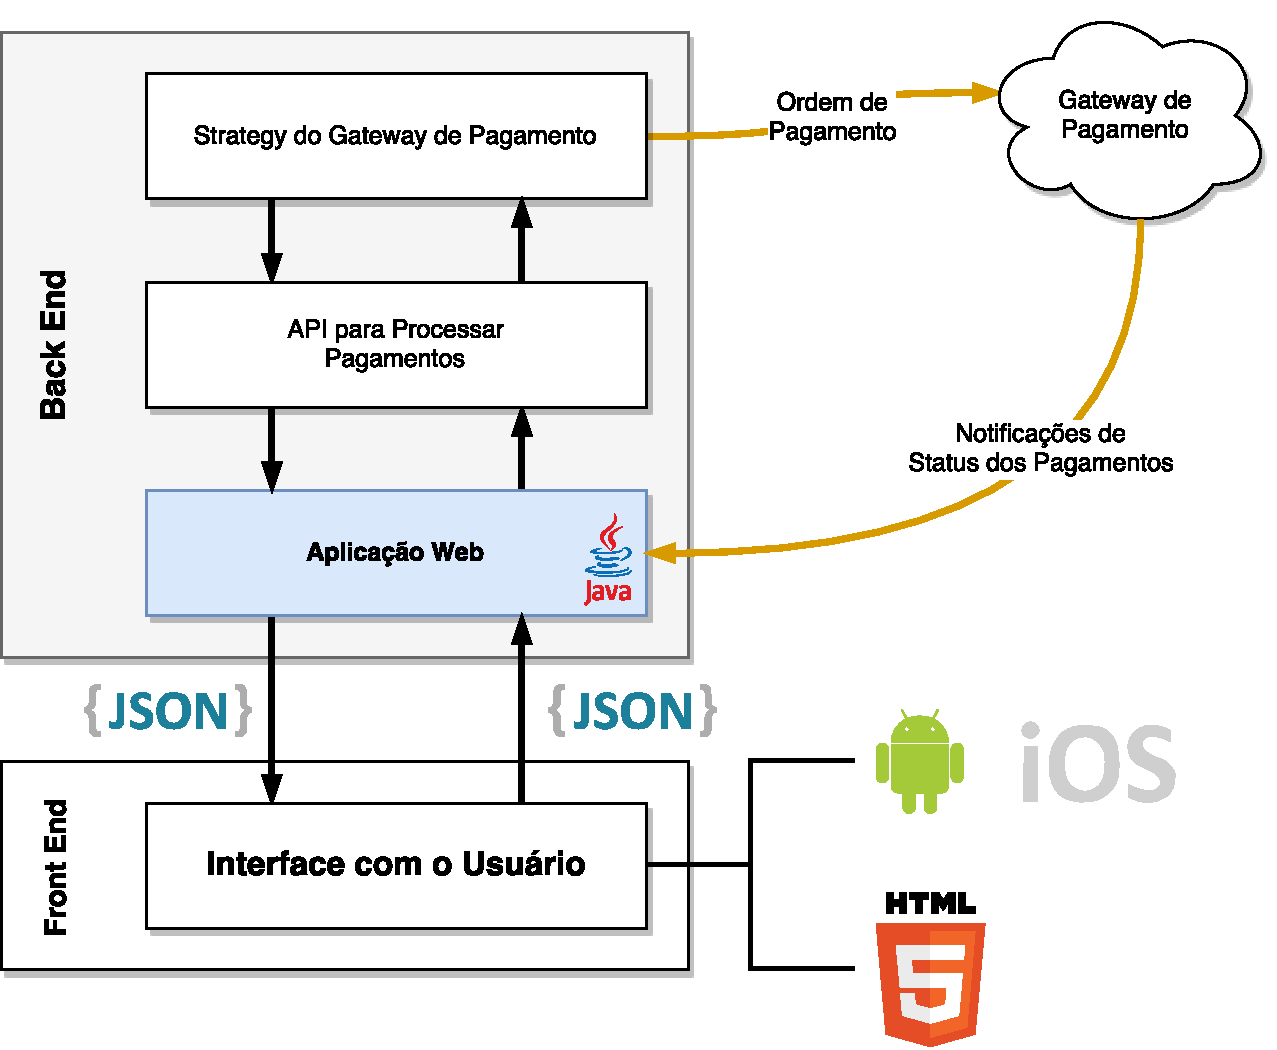
\includegraphics[scale=0.7]{imagens/ajudaAi-arquitetura.pdf}
  \legend{Fonte: Elaborado pelo Autor}
\end{figure}

Requisições são feitas ao sistema de duas origens: A interface com o usuário e os \emph{gateways} de pagamento. As requisições feitas pela interface são padronizadas como JSON a fim de facilitar a criação de aplicações modernas e diminuir o tráfego de dados. Já requisições feitas pelos \emph{gateways} são suportadas em XML, JSON, \emph{x-www-form-urlencoded} (formulário HTML padrão) e \emph{form-data} (formulário HTML com dados longos, definido pelo RFC2388).

Um dos diferenciais do Ajuda.Ai é o suporte a diferentes \emph{gateways} de pagamento. Isso dá flexibilidade a instituição para usar o \emph{gateway} mais adequado a mesma. Para implementação foi utilizado o Padrão de Projeto de Software \emph{Strategy}, como ilustrado na Figura \ref{fig:uml_strategy}. Este Padrão de Projeto é definido por uma família de algoritmos encapsulados e que podem ser trocados dentro da família de objetos \cite{gamma1995design}.

\begin{figure}[H]
	\caption{\label{fig:uml_strategy}Estrutura dos Processadores de Pagamento}
    \centering
	\begin{tikzpicture}
		\umlclass[type=interface]{PaymentGateway}{}{
			+ createPayment() : Payment \\
            + processEvent() : PaymentEvent}
        \umlclass[x=-3.5, y=-4]{MoipPaymentGateway}{}{
			+ createPayment() : Payment \\
            + processEvent() : PaymentEvent}
        \umlclass[x=3.5, y=-4]{PagSeguroPaymentGateway}{}{
			+ createPayment() : Payment \\
            + processEvent() : PaymentEvent}
        \umlsimpleclass[x=-3, y=3]{InstitutionController}
        \umlsimpleclass[x=3, y=3]{TransactionNotificationController}
        \umlcompo[very thick]{InstitutionController}{PaymentGateway}
        \umlcompo[very thick]{TransactionNotificationController}{PaymentGateway}
        \umlimpl[very thick]{MoipPaymentGateway}{PaymentGateway}
        \umlimpl[very thick]{PagSeguroPaymentGateway}{PaymentGateway}
  \end{tikzpicture}
  \legend{Fonte: Elaborado pelo Autor}
\end{figure}

Cada implementação de \emph{gateway} de pagamento suportado implementa a interface \codigo{PaymentGateway}. Esta interface tem dois métodos:

\begin{lista}
  \item \textbf{\codigo{createPayment()}}: Cria uma ordem de pagamento junto ao \emph{gateway} de pagamento. Esse método tem liberdade de redirecionar o usuário para o sistema do \emph{gateway} (MoIP e a maioria dos gateways nacionais) ou enviar algum pedaço de informação, como JSON, como resposta ao usuário (PayPal + JavaScript para pagamento na própria página). Este método deve retornar um objeto \codigo{Payment} para ser persistido a fim de acompanhar o andamento do pagamento;

  \item \textbf{\codigo{processPayment()}}: \emph{Gateways} de pagamento enviam requisições de volta ao sistema informando sobre o status de um determinado pagamento feito na plataforma deles. Esse método é encarregado de processar essas mudanças de estado no pagamento. Este método deve retornar um objeto \codigo{PaymentEvent} que indica de forma padronizada o que aconteceu com este pagamento.
\end{lista}

Ao criar uma ordem de pagamento através de \codigo{createPayment()} a classe que a criou retorna um objeto \codigo{Payment} para ser persistido. Esse objeto, além de padronizar as informações relevantes dos pagamentos, guarda consigo a estratégia (serviço de pagamento) utilizada para criar a ordem de pagamento. Essa informação é usada futuramente quando o sistema recebe uma notificação de estado de pagamento.

Uma vantagem da utilização do padrão \emph{Strategy} é que diferentes usos de um mesmo \emph{gateway} podem ser facilmente implementados. Por exemplo, o \emph{gateway} MoIP oferece várias formas para criar ordens de pagamento. Três delas são interessantes para o que o Ajuda.Ai propõe:

\begin{lista}
  \item \textbf{Ordem de pagamento via e-mail:} O MoIP envia um e-mail para o usuário onde, na conveniência do mesmo, ele tem 30 dias para efetuar o pagamento da forma como preferir;
  \item \textbf{\emph{Check-out} Clássico:} O usuário é redirecionado para o \emph{Gateway} onde ele selecionará forma de pagamento e fará todo o processo de pagamento antes de voltar ao Ajuda.Ai --- Essa forma está disponível em todos os \emph{gateways} e é a forma preferencial de se fazer a interação de pagamento junto ao usuário;
  \item \textbf{\emph{Check-out} Transparente:} O usuário preenche tudo no próprio sistema o qual junto ao \emph{gateway} e através de \emph{webservices} faz uma ordem de pagamento e processamento de pagamento --- Esta forma está disponível em quase todos os \emph{gateways}.
\end{lista}

O Ajuda.Ai se utiliza da segunda forma demonstrada, o \emph{Check-Out} Clássico, pois é suportada por todos os \emph{gateways} e recomendada pelos mesmos por prover um ambiente seguro e que os usuários demonstram maior confiança ao partilhar dados sigilosos e pessoais como números de cartão de crédito e CPF. Esse processo de pagamento será detalhado na próxima subseção.





\subsection{Processo Comum de Pagamentos Online} \label{sec:ajudaai:processo_pagamento}

A ilustração da Figura \ref{fig:gateway} mostra o fluxo de criação e processamento de pagamento comum a maioria dos \emph{gateways} atualmente no mercado. Todo o processo acontece entre duas entidades que são o Sistema, que é o sistema que irá gerar as ordens de pagamento e ser notificado do andamento dos pagamentos, e o próprio \emph{Gateway} de Pagamento. O processo começa com a geração de uma ordem de pagamento junto ao \emph{gateway}, a qual pode ser feita de duas maneiras:

\begin{lista}
	\item \textbf{Pagamento Normal}: Nessa modalidade, o Sistema faz um HTTP POST com dados sobre o que está sendo comprado ao \emph{Gateway} e o usuário é redirecionado até uma página do próprio \emph{Gateway} de pagamento. Esse é o modo recomendado pelos \emph{Gateways}, pois os \emph{Gateways} podem servir a página de forma segura, protegida através de certificados digitais confiáveis, com uma interface de usuário adequada. Segundo os \emph{Gateways}, os clientes ficam mais propensos a concluir a compra quando o pagamento utiliza esse formato, pois os mesmos confiam na marca do \emph{Gateway} e na segurança do ambiente;
	\item \textbf{Pagamento Transparente}: Nessa modalidade, todos os dados do pagamento são preenchidos em uma interface provida pelo próprio Sistema e enviados de forma segura ao \emph{Gateway} de Pagamento, o qual imediatamente cria e inicia o processamento do pagamento da uma ordem de pagamento.
\end{lista}

\begin{figure}[H]
	\caption{\label{fig:gateway}Fluxo de um Pagamento via \emph{Gateway} de Pagamento}
    \centering
    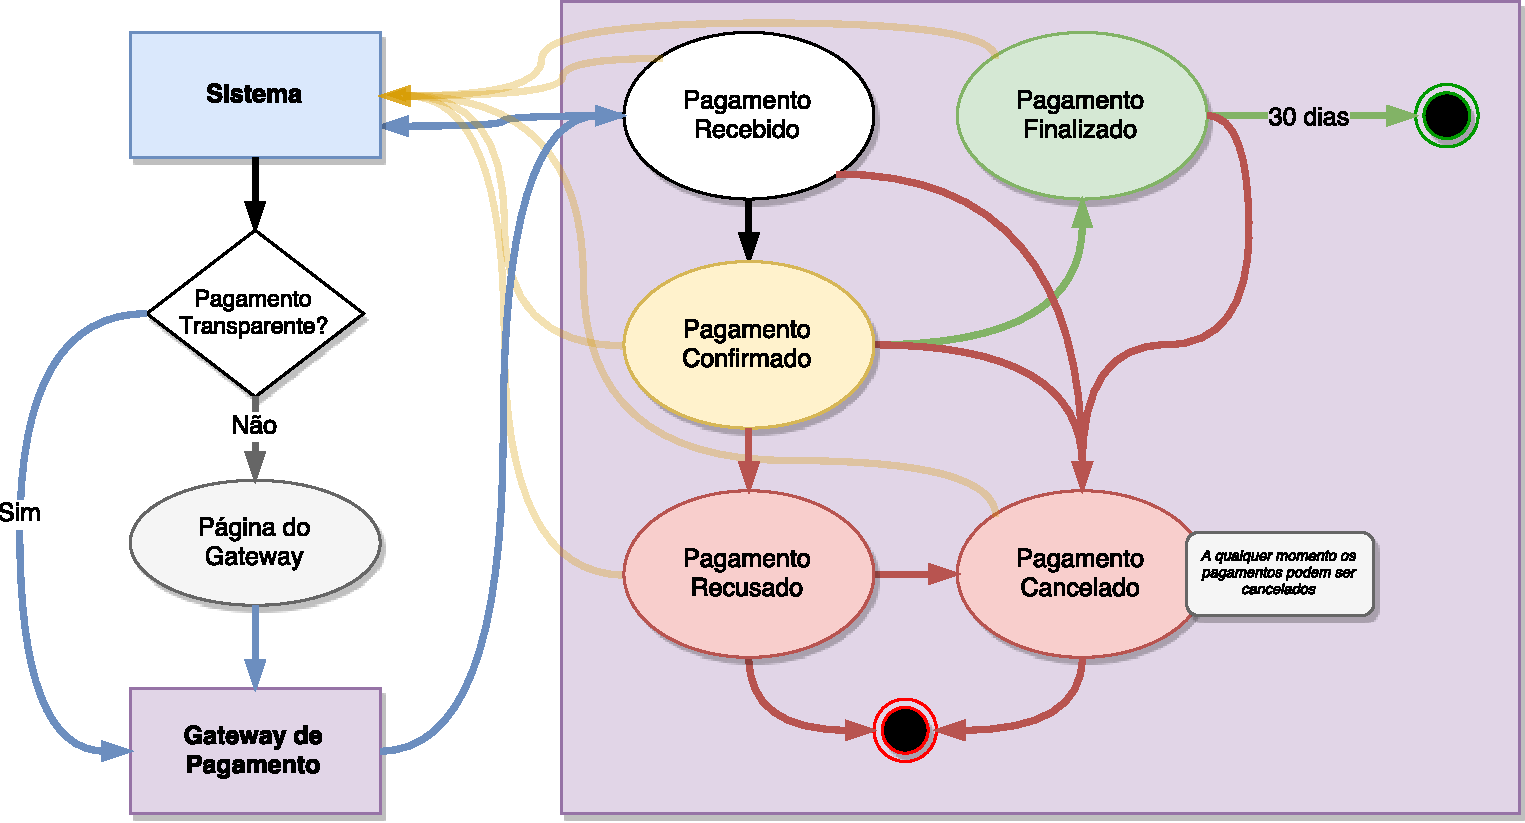
\includegraphics[scale=0.575]{imagens/processo_gateway.pdf}
    \legend{Fonte: Elaborado pelo Autor}
\end{figure}

O Ajuda.Ai faz uso da primeira maneira, o Pagamento Normal, onde o usuário é redirecionado ao \emph{Gateway}. Após a criação do pedido de pagamento e o preenchimento das informações necessárias, como dados pessoais, CPF e outros, o \emph{Gateway} cria um pagamento em seu sistema, e a partir desse ponto começa a máquina de estados do \emph{Gateway}. A máquina apresentada é uma simplificação e normalização do que ocorre na maioria dos \emph{Gateways}.

Na ilustração da Figura \ref{fig:gateway} as setas de cor azul representam o fluxo como visto pelo usuário do Sistema. O usuário preenche algumas informações no próprio Sistema ou no \emph{Gateway} e, ao enviar, é feita a ordem de pagamento e o usuário é redirecionado de volta ao Sistema em uma página de ``Obrigado''. Esta é uma página do Sistema para onde o \emph{Gateway} irá redirecionar o usuário ao final do fluxo de criação da ordem de pagamento.

Ao criar uma ordem de pagamento, inicia-se uma máquina de estados do pagamento que muda de acordo com o andamento do pagamento ou ações do usuário. Durante os estados na máquina de estados do \emph{Gateway} cada alteração de estado resulta em uma notificação ao sistema, representadas pelas setas na cor laranja. Esse comportamento é típico do padrão de projetos \emph{Event Notifier}, também conhecido como \emph{Publish-Subscribe} ou \emph{Pub-Sub}. Esse padrão de projeto permite que dois sistemas comuniquem eventos entre si sem necessariamente ter conhecimento um do outro \cite{gupta2000event}.

Como parte da implementação deste padrão de projeto, os \emph{gateways} de pagamento provêm alguma maneira de configurar quais URL do Sistema deverá ser chamada para receber as notificações geradas pelas trocas de estado. Na ilustração da Figura \ref{fig:config_moip} está a configuração desta opção no sistema do \emph{gateway} MoIP.

\begin{figure}[H]
	\caption{\label{fig:config_moip}Configuração de Notificação do \emph{Gateway} de Pagamento MoIP}
    \centering
    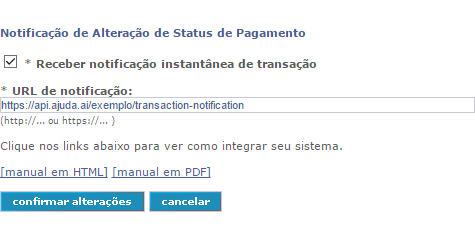
\includegraphics[scale=0.85]{imagens/config-moip.png}
    \legend{Fonte: Elaborado pelo Autor}
\end{figure}

A cada alteração de estado do pagamento uma requisição específica a URL configurada será feita. Para facilitar a configuração dos vários diferentes \emph{gateways} no mercado a URL do Ajuda.Ai a ser configurada neles é padronizada, mudando apenas um parâmetro que representa qual \emph{gateway} fará requisições a URL. Na ilustração da Figura \ref{fig:config_moip} temos a URL referente ao MoIP.

Uma vez criado um pagamento junto ao \emph{gateway} ele deve ser confirmado. Esse estado é mais evidente quando o pagamento é feito por Boleto Bancário, pois o mesmo demora até 3 dias úteis para ser processado pelo banco e o retorno dado ao \emph{gateway}. Em pagamentos via cartão de crédito a confirmação é simplesmente o recebimento da requisição de crédito através dos sistemas da mesma, o que quase sempre é imediato.

Na confirmação o \emph{gateway} é informado do sucesso ou falha na execução do pagamento. Caso o pagamento tenha sido feito sem problemas, ele vai para o estado Finalizado, vai para Recusado. Como explicitado na Figura \ref{fig:gateway}, a praticamente qualquer momento do processo o usuário poderá Cancelar o pagamento. Apenas após 30 dias no estado Finalizado, o cancelamento da operação fica indisponível, entretanto este prazo pode mudar de acordo com o \emph{gateway}. Vale salientar também, que apenas após este prazo o dinheiro estará disponível para resgate pela instituição.

Cada mudança de estado resulta em uma chamada a URL configurada juntamente a um pacote de informações sobre o estado atual do pagamento. Cada \emph{Gateway} envia informações distintas, mas bastante semelhantes. A mais importante delas é o que é chamado de ID do Cliente que é um número especificado pelo Sistema e que será vinculado aquele pagamento. Este campo deve ser utilizado pelo Sistema para identificar internamente o que está sendo pago. O Ajuda.Ai utiliza este campo para manter o ID do objeto \codigo{Payment} gerado no início do processo a fim de manter o estado do pagamento e vincular a instituição correspondente.





\section{API REST Web} \label{sec:ajudaai:api}

%Você pode falar sobre a necessidade de se documentar a API, de forma a dirimir dúvidas de implementações que consumirem os serviços. Pode falar que não existe um padrão, mas que neste trabalho você usou o formato x, y, z e através dele é possível ter uma microvisão da coisa toda.

Para facilitar o desenvolvimento de diferentes interfaces com o usuário e demais consumidores da API e prevenir dúvidas quanto a mesma e seu funcionamento a API REST Web do \emph{backend} do projeto Ajuda.Ai foi documentada. Esses são os métodos da API que estão disponíveis para todos os clientes, porém alguns necessitam de login. Os métodos que não necessitam de login são classificados como métodos públicos.

Apesar da importância de uma boa documentação ainda não há um padrão estabelecido para a forma de documentar APIs REST Web. Por esse motivo este trabalho se utiliza do formato proposto por Irene Ros\cite{blog:bocoup}, diretora da Bocoup, empresa de consultoria referência em desenvolvimento REST Web e produtora de diversas ferramentas de código fonte aberto para se trabalhar com REST Web e \emph{Front-end}. A seguir está a API REST Web disponibilizada pelo Ajuda.Ai. Todos os parâmetros são obrigatórios, a menos que especificado que seja opcional. Parâmetros que fazem parte da própria URL são indicados com um sinal de dois-pontos no início de seu nome:

\begin{caixa}{Autenticação do Usuário}{}

Retorna informações sobre o usuário logado. Usado para, além de pegar informações sobre o usuário logado, manter a Sessão de autenticação ativa.

\begin{itemize}
\item \textbf{URL}
	\begin{itemize}
		\item \codigo{/auth/login}
	\end{itemize}

\item \textbf{Método}
	\begin{itemize}
		\item \codigo{POST}
	\end{itemize}

\item \textbf{Parâmetros}
	\begin{itemize}
    	\item Nenhum Parâmetro
	\end{itemize}

\item \textbf{Parâmetros de Dados}
	\begin{itemize}
        \item \codigo{username=String} Nome de usuário ou E-mail do Usuário que quer se autenticar
        \item \codigo{password=String} Senha do Usuário
	\end{itemize}

\item \textbf{Resposta de Sucesso}
	\begin{itemize}
		\item \textbf{Código:} \codigo{200 OK} \\ \textbf{Conteúdo:} JSON de um objeto \codigo{User} apenas com os campos \codigo{id}, \codigo{username}, \codigo{email}, \codigo{firstname} e \codigo{lastname} do Usuário logado.
	\end{itemize}

\item \textbf{Resposta de Erro}
	\begin{itemize}
		\item \textbf{Código:} \codigo{200 OK} \\ \textbf{Conteúdo:} \codigo{Array} com os erros de autenticação \\ \textbf{Motivo:} Usuário ou senha incorretos.
        \item \textbf{Código:} \codigo{405 METHOD NOT ALLOWED} \\ \textbf{Conteúdo:} Nenhum \\ \textbf{Motivo:} A chamada HTTP não utilizou o método \codigo{POST}.
	\end{itemize}

\end{itemize}
\end{caixa}

%%%%%%%%%%%%%%%%%%%%%%%%%%%%%%%%%%%%%%%%%%%%%%%%%%%%%%%%%%%%%%%%%%%%%%%%%
%%%%%%%%%%%%%%%%%%%%%%%%%%%%%%%%%%%%%%%%%%%%%%%%%%%%%%%%%%%%%%%%%%%%%%%%%
%%%%%%%%%%%%%%%%%%%%%%%%%%%%%%%%%%%%%%%%%%%%%%%%%%%%%%%%%%%%%%%%%%%%%%%%%
%%%%%%%%%%%%%%%%%%%%%%%%%%%%%%%%%%%%%%%%%%%%%%%%%%%%%%%%%%%%%%%%%%%%%%%%%

\begin{caixa}{Dados do Usuário Logado}{}

Retorna informações sobre o usuário logado. Usado para, além de pegar informações sobre o usuário logado, manter a Sessão de autenticação ativa. A sessão de autenticação dura por 30 minutos após a última requisição a API.

\begin{itemize}
\item \textbf{URL}
	\begin{itemize}
		\item \codigo{/profile/me}
	\end{itemize}

\item \textbf{Método}
	\begin{itemize}
		\item \codigo{GET}
	\end{itemize}

\item \textbf{Parâmetros}
	\begin{itemize}
		\item Nenhum Parâmetro
	\end{itemize}

\item \textbf{Parâmetros de Dados}
	\begin{itemize}
		\item Nenhum Parâmetro
	\end{itemize}

\item \textbf{Resposta de Sucesso}
	\begin{itemize}
		\item \textbf{Código:} \codigo{200 OK} \\ \textbf{Conteúdo:} JSON do objeto \codigo{User} do usuário logado, apenas com os campos \codigo{id}, \codigo{username}, \codigo{email}, \codigo{firstname} e \codigo{lastname}.
	\end{itemize}

\item \textbf{Resposta de Erro}
	\begin{itemize}
		\item \textbf{Código:} \codigo{401 UNAUTHORIZED} \\ \textbf{Conteúdo:} Nenhum \\ \textbf{Motivo:} Não há um Usuário logado
        \item \textbf{Código:} \codigo{405 METHOD NOT ALLOWED} \\ \textbf{Conteúdo:} Nenhum \\ \textbf{Motivo:} A chamada HTTP não utilizou o método \codigo{GET}.
	\end{itemize}

\end{itemize}
\end{caixa}

%%%%%%%%%%%%%%%%%%%%%%%%%%%%%%%%%%%%%%%%%%%%%%%%%%%%%%%%%%%%%%%%%%%%%%%%%
%%%%%%%%%%%%%%%%%%%%%%%%%%%%%%%%%%%%%%%%%%%%%%%%%%%%%%%%%%%%%%%%%%%%%%%%%
%%%%%%%%%%%%%%%%%%%%%%%%%%%%%%%%%%%%%%%%%%%%%%%%%%%%%%%%%%%%%%%%%%%%%%%%%
%%%%%%%%%%%%%%%%%%%%%%%%%%%%%%%%%%%%%%%%%%%%%%%%%%%%%%%%%%%%%%%%%%%%%%%%%

\begin{caixa}{Dados de um Usuário}{}

Retorna informações sobre o usuário especificado a partir de seu nome de usuário.

\begin{itemize}
\item \textbf{URL}
	\begin{itemize}
		\item \codigo{/profile/:username}
	\end{itemize}

\item \textbf{Método}
	\begin{itemize}
		\item \codigo{GET}
	\end{itemize}

\item \textbf{Parâmetros}
	\begin{itemize}
		\item \codigo{username=String} - \textbf{(opcional se \codigo{id} for especificado)} Nome único de usuário
	\end{itemize}

\item \textbf{Parâmetros de Dados}
	\begin{itemize}
		\item \codigo{id=Integer} - Identificador do usuário
	\end{itemize}

\item \textbf{Resposta de Sucesso}
	\begin{itemize}
		\item \textbf{Código:} \codigo{200 OK} \\ \textbf{Conteúdo:} JSON do objeto \codigo{User} do usuário encontrado, apenas com os campos \codigo{id}, \codigo{username}, \codigo{firstname} e \codigo{lastname}.
	\end{itemize}

\item \textbf{Resposta de Erro}
	\begin{itemize}
		\item \textbf{Código:} \codigo{404 NOT FOUND} \\ \textbf{Conteúdo:} Nenhum \\ \textbf{Motivo:} Usuário não existe
        \item \textbf{Código:} \codigo{405 METHOD NOT ALLOWED} \\ \textbf{Conteúdo:} Nenhum \\ \textbf{Motivo:} A chamada HTTP não utilizou o método \codigo{GET}.
	\end{itemize}

\end{itemize}
\end{caixa}

%%%%%%%%%%%%%%%%%%%%%%%%%%%%%%%%%%%%%%%%%%%%%%%%%%%%%%%%%%%%%%%%%%%%%%%%%
%%%%%%%%%%%%%%%%%%%%%%%%%%%%%%%%%%%%%%%%%%%%%%%%%%%%%%%%%%%%%%%%%%%%%%%%%
%%%%%%%%%%%%%%%%%%%%%%%%%%%%%%%%%%%%%%%%%%%%%%%%%%%%%%%%%%%%%%%%%%%%%%%%%
%%%%%%%%%%%%%%%%%%%%%%%%%%%%%%%%%%%%%%%%%%%%%%%%%%%%%%%%%%%%%%%%%%%%%%%%%

\begin{caixa}{Dados de uma Instituição}{}

Retorna todos os dados de uma Instituição.

\begin{itemize}
\item \textbf{URL}
	\begin{itemize}
		\item \codigo{/institution/:slug}
	\end{itemize}

\item \textbf{Método}
	\begin{itemize}
		\item \codigo{GET}
	\end{itemize}

\item \textbf{Parâmetros}
	\begin{itemize}
		\item \codigo{slug=String} - Nome da URL da Instituição
	\end{itemize}

\item \textbf{Parâmetros de Dados}
	\begin{itemize}
		\item Nenhum Parâmetro
	\end{itemize}

\item \textbf{Resposta de Sucesso}
	\begin{itemize}
		\item \textbf{Código:} \codigo{200 OK} \\ \textbf{Conteúdo:} JSON com os dados da Instituição
	\end{itemize}

\item \textbf{Resposta de Erro}
	\begin{itemize}
		\item \textbf{Código:} \codigo{404 NOT FOUND} \\ \textbf{Conteúdo:} Nenhum \\ \textbf{Motivo:} Instituição não existe
        \item \textbf{Código:} \codigo{405 METHOD NOT ALLOWED} \\ \textbf{Conteúdo:} Nenhum \\ \textbf{Motivo:} A chamada HTTP não utilizou o método \codigo{GET}.
	\end{itemize}

\end{itemize}
\end{caixa}

%%%%%%%%%%%%%%%%%%%%%%%%%%%%%%%%%%%%%%%%%%%%%%%%%%%%%%%%%%%%%%%%%%%%%%%%%
%%%%%%%%%%%%%%%%%%%%%%%%%%%%%%%%%%%%%%%%%%%%%%%%%%%%%%%%%%%%%%%%%%%%%%%%%
%%%%%%%%%%%%%%%%%%%%%%%%%%%%%%%%%%%%%%%%%%%%%%%%%%%%%%%%%%%%%%%%%%%%%%%%%
%%%%%%%%%%%%%%%%%%%%%%%%%%%%%%%%%%%%%%%%%%%%%%%%%%%%%%%%%%%%%%%%%%%%%%%%%

\begin{caixa}{Dados de uma Instituição escolhida Aleatoriamente}{}

Retorna todos os dados de uma Instituição escolhida aleatoriamente.

\begin{itemize}
\item \textbf{URL}
	\begin{itemize}
		\item \codigo{/institution/random}
	\end{itemize}

\item \textbf{Método}
	\begin{itemize}
		\item \codigo{GET}
	\end{itemize}

\item \textbf{Parâmetros}
	\begin{itemize}
		\item Nenhum Parâmetro
	\end{itemize}

\item \textbf{Parâmetros de Dados}
	\begin{itemize}
		\item Nenhum Parâmetro
	\end{itemize}

\item \textbf{Resposta de Sucesso}
	\begin{itemize}
		\item \textbf{Código:} \codigo{200 OK} \\ \textbf{Conteúdo:} JSON com os dados de uma Instituição
	\end{itemize}

\item \textbf{Resposta de Erro}
	\begin{itemize}
		\item \textbf{Código:} \codigo{404 NOT FOUND} \\ \textbf{Conteúdo:} Nenhum \\ \textbf{Motivo:} Não há nenhuma instituição cadastrada no banco de dados
        \item \textbf{Código:} \codigo{405 METHOD NOT ALLOWED} \\ \textbf{Conteúdo:} Nenhum \\ \textbf{Motivo:} A chamada HTTP não utilizou o método \codigo{GET}.
	\end{itemize}

\end{itemize}
\end{caixa}

%%%%%%%%%%%%%%%%%%%%%%%%%%%%%%%%%%%%%%%%%%%%%%%%%%%%%%%%%%%%%%%%%%%%%%%%%
%%%%%%%%%%%%%%%%%%%%%%%%%%%%%%%%%%%%%%%%%%%%%%%%%%%%%%%%%%%%%%%%%%%%%%%%%
%%%%%%%%%%%%%%%%%%%%%%%%%%%%%%%%%%%%%%%%%%%%%%%%%%%%%%%%%%%%%%%%%%%%%%%%%
%%%%%%%%%%%%%%%%%%%%%%%%%%%%%%%%%%%%%%%%%%%%%%%%%%%%%%%%%%%%%%%%%%%%%%%%%

\begin{caixa}{Lista de Instituições escolhidas Aleatoriamente}{}

Retorna uma lista de até 12 Instituições escolhidas aleatoriamente. Útil para exibir Instituições na Página Inicial.

\begin{itemize}
\item \textbf{URL}
	\begin{itemize}
		\item \codigo{/institution/random-list}
	\end{itemize}

\item \textbf{Método}
	\begin{itemize}
		\item \codigo{GET}
	\end{itemize}

\item \textbf{Parâmetros}
	\begin{itemize}
		\item Nenhum Parâmetro
	\end{itemize}

\item \textbf{Parâmetros de Dados}
	\begin{itemize}
		\item Nenhum Parâmetro
	\end{itemize}

\item \textbf{Resposta de Sucesso}
	\begin{itemize}
		\item \textbf{Código:} \codigo{200 OK} \\ \textbf{Conteúdo:} JSON com um \codigo{Array} com dados de Instituições escolhidas aleatoriamente. Máximo de 12 instituições.
	\end{itemize}

\item \textbf{Resposta de Erro}
	\begin{itemize}
		\item \textbf{Código:} \codigo{404 NOT FOUND} \\ \textbf{Conteúdo:} Nenhum \\ \textbf{Motivo:} Não há nenhuma instituição cadastrada no banco de dados
        \item \textbf{Código:} \codigo{405 METHOD NOT ALLOWED} \\ \textbf{Conteúdo:} Nenhum \\ \textbf{Motivo:} A chamada HTTP não utilizou o método \codigo{GET}.
	\end{itemize}

\end{itemize}
\end{caixa}

%%%%%%%%%%%%%%%%%%%%%%%%%%%%%%%%%%%%%%%%%%%%%%%%%%%%%%%%%%%%%%%%%%%%%%%%%
%%%%%%%%%%%%%%%%%%%%%%%%%%%%%%%%%%%%%%%%%%%%%%%%%%%%%%%%%%%%%%%%%%%%%%%%%
%%%%%%%%%%%%%%%%%%%%%%%%%%%%%%%%%%%%%%%%%%%%%%%%%%%%%%%%%%%%%%%%%%%%%%%%%
%%%%%%%%%%%%%%%%%%%%%%%%%%%%%%%%%%%%%%%%%%%%%%%%%%%%%%%%%%%%%%%%%%%%%%%%%

\begin{caixa}{Estatísticas de Doações}{}

Retorna quantas doações a Instituição recebeu e o valor total das mesmas.

\begin{itemize}
\item \textbf{URL}
	\begin{itemize}
		\item \codigo{/institution/:slug/donation-stats}
	\end{itemize}

\item \textbf{Método}
	\begin{itemize}
		\item \codigo{GET}
	\end{itemize}

\item \textbf{Parâmetros}
	\begin{itemize}
		\item \codigo{slug=String} - Nome da URL da Instituição
	\end{itemize}

\item \textbf{Parâmetros de Dados}
	\begin{itemize}
		\item Nenhum Parâmetro
	\end{itemize}

\item \textbf{Resposta de Sucesso}
	\begin{itemize}
		\item \textbf{Código:} \codigo{200 OK} \\ \textbf{Conteúdo:} JSON no seguinte formato: \\ \codigo{\{ count: Integer, value: Integer \}} - O valor deve ser dividido por 100 para ser exibido adequadamente.
	\end{itemize}

\item \textbf{Resposta de Erro}
	\begin{itemize}
		\item \textbf{Código:} \codigo{404 NOT FOUND} \\ \textbf{Conteúdo:} Nenhum \\ \textbf{Motivo:} Instituição não existe
        \item \textbf{Código:} \codigo{405 METHOD NOT ALLOWED} \\ \textbf{Conteúdo:} Nenhum \\ \textbf{Motivo:} A chamada HTTP não utilizou o método \codigo{GET}.
	\end{itemize}

\end{itemize}
\end{caixa}

%%%%%%%%%%%%%%%%%%%%%%%%%%%%%%%%%%%%%%%%%%%%%%%%%%%%%%%%%%%%%%%%%%%%%%%%%
%%%%%%%%%%%%%%%%%%%%%%%%%%%%%%%%%%%%%%%%%%%%%%%%%%%%%%%%%%%%%%%%%%%%%%%%%
%%%%%%%%%%%%%%%%%%%%%%%%%%%%%%%%%%%%%%%%%%%%%%%%%%%%%%%%%%%%%%%%%%%%%%%%%
%%%%%%%%%%%%%%%%%%%%%%%%%%%%%%%%%%%%%%%%%%%%%%%%%%%%%%%%%%%%%%%%%%%%%%%%%

\begin{caixa}{Doação - Passo 01: Registrar o Pagamento}{}

Inicia o processo de doação gravando os dados da mesma no Ajuda.Ai. Posteriormente o usuário deverá ser redirecionando para o \emph{gateway} de pagamento vinculado a Instituição através do método \codigo{/pagar/:id}.

\begin{itemize}
\item \textbf{URL}
	\begin{itemize}
		\item \codigo{/institution/:slug/doar}
	\end{itemize}

\item \textbf{Método}
	\begin{itemize}
		\item \codigo{POST}
	\end{itemize}

\item \textbf{Parâmetros}
	\begin{itemize}
		\item \codigo{slug=String} - Nome da URL da Instituição
	\end{itemize}

\item \textbf{Parâmetros de Dados}
	\begin{itemize}
        \item \codigo{value=Integer} - Valor da Doação como um Inteiro (10000 = \$100,00)
        \item \codigo{name=String} - \textbf{(opcional se feito o login)} Nome Completo do Doador
        \item \codigo{email=String} - \textbf{(opcional se feito o login)} E-mail do Doador
        %\item \codigo{anonymous=Boolean} - Doação anônima?
        \item \codigo{addcosts=Boolean} - Adicionar custos operacionais do Gateway ao valor da doação?
        \item \codigo{addcoststype=Integer} - Tipo de pagamento que será utilizado (para cálculo do custo operacional)
	\end{itemize}

\item \textbf{Resposta de Sucesso}
	\begin{itemize}
		\item \textbf{Código:} \codigo{200 OK} \\ \textbf{Conteúdo:} Objeto \codigo{Payment} com os dados do pagamento criado
	\end{itemize}

\item \textbf{Resposta de Erro}
	\begin{itemize}
		\item \textbf{Código:} \codigo{404 NOT FOUND} \\ \textbf{Conteúdo:} Nenhum \\ \textbf{Motivo:} Instituição não existe
        \item \textbf{Código:} \codigo{405 METHOD NOT ALLOWED} \\ \textbf{Conteúdo:} Nenhum \\ \textbf{Motivo:} A chamada HTTP não utilizou o método \codigo{POST}.
	\end{itemize}

\end{itemize}
\end{caixa}

%%%%%%%%%%%%%%%%%%%%%%%%%%%%%%%%%%%%%%%%%%%%%%%%%%%%%%%%%%%%%%%%%%%%%%%%%
%%%%%%%%%%%%%%%%%%%%%%%%%%%%%%%%%%%%%%%%%%%%%%%%%%%%%%%%%%%%%%%%%%%%%%%%%
%%%%%%%%%%%%%%%%%%%%%%%%%%%%%%%%%%%%%%%%%%%%%%%%%%%%%%%%%%%%%%%%%%%%%%%%%
%%%%%%%%%%%%%%%%%%%%%%%%%%%%%%%%%%%%%%%%%%%%%%%%%%%%%%%%%%%%%%%%%%%%%%%%%

\begin{caixa}{Doação - Passo 02: Redirecionamento ao \emph{Gateway}}{}

Continua o processo de doação redirecionando o usuário para o \emph{gateway} de pagamento vinculado ao \codigo{Payment} especificado.

\begin{itemize}
\item \textbf{URL}
	\begin{itemize}
		\item \codigo{/pagar/:id}
	\end{itemize}

\item \textbf{Método}
	\begin{itemize}
		\item \codigo{GET}
	\end{itemize}

\item \textbf{Parâmetros}
	\begin{itemize}
		\item \codigo{id=UUID} - Identificador do pagamento (UUID)
	\end{itemize}

\item \textbf{Parâmetros de Dados}
	\begin{itemize}
        \item Nenhum Parâmetro
	\end{itemize}

\item \textbf{Resposta de Sucesso}
	\begin{itemize}
		\item \textbf{Código:} \codigo{302 MOVED TEMPORARILY} \\ \textbf{Conteúdo:} Nenhum
	\end{itemize}

\item \textbf{Resposta de Erro}
	\begin{itemize}
		\item \textbf{Código:} \codigo{404 NOT FOUND} \\ \textbf{Conteúdo:} Nenhum \\ \textbf{Motivo:} Pagamento não existe
        \item \textbf{Código:} \codigo{409 CONFLICT} \\ \textbf{Conteúdo:} Nenhum \\ \textbf{Motivo:} Notificações do \emph{Gateway} informam que este pagamento já está ou já foi processado.
        \item \textbf{Código:} \codigo{405 METHOD NOT ALLOWED} \\ \textbf{Conteúdo:} Nenhum \\ \textbf{Motivo:} A chamada HTTP não utilizou o método \codigo{GET}.
	\end{itemize}

\end{itemize}
\end{caixa}

%%%%%%%%%%%%%%%%%%%%%%%%%%%%%%%%%%%%%%%%%%%%%%%%%%%%%%%%%%%%%%%%%%%%%%%%%
%%%%%%%%%%%%%%%%%%%%%%%%%%%%%%%%%%%%%%%%%%%%%%%%%%%%%%%%%%%%%%%%%%%%%%%%%
%%%%%%%%%%%%%%%%%%%%%%%%%%%%%%%%%%%%%%%%%%%%%%%%%%%%%%%%%%%%%%%%%%%%%%%%%
%%%%%%%%%%%%%%%%%%%%%%%%%%%%%%%%%%%%%%%%%%%%%%%%%%%%%%%%%%%%%%%%%%%%%%%%%

\begin{caixa}{\emph{Posts} de uma Instituição}{}

Retorna uma lista de tamanho limitado com os \emph{posts} de uma Instituição.

\begin{itemize}
\item \textbf{URL}
	\begin{itemize}
		\item \codigo{/institution/:slug/posts}
	\end{itemize}

\item \textbf{Método}
	\begin{itemize}
		\item GET
	\end{itemize}

\item \textbf{Parâmetros}
	\begin{itemize}
		\item \codigo{slug=String} - Nome de URL da Instituição
	\end{itemize}

\item \textbf{Parâmetros de Dados}
	\begin{itemize}
		\item \codigo{size=Integer} - \textbf{(opcional)} Quantidade de Itens na lista. Padrão: \codigo{10}. Máximo: \codigo{50}.
        \item \codigo{offset=Integer} - \textbf{(opcional)} Primeiro item da lista. Padrão: \codigo{0}.
	\end{itemize}

\item \textbf{Resposta de Sucesso}
	\begin{itemize}
		\item \textbf{Código:} \codigo{200 OK} \\ \textbf{Conteúdo:} JSON no seguinte formato: \\ \codigo{\{ size: Integer, total: Integer, offset: Integer, items: [InstitutionPost] \}} \\
        Nota: os \emph{posts} terão apenas os campos id, slug, titulo, subtitulo, criador e data e hora de criação.
	\end{itemize}

\item \textbf{Resposta de Erro}
	\begin{itemize}
		\item \textbf{Código:} \codigo{404 NOT FOUND} \\ \textbf{Conteúdo:} Nenhum \\ \textbf{Motivo:} Instituição não existe
        \item \textbf{Código:} \codigo{405 METHOD NOT ALLOWED} \\ \textbf{Conteúdo:} Nenhum \\ \textbf{Motivo:} A chamada HTTP não utilizou o método \codigo{GET}.
	\end{itemize}

\end{itemize}
\end{caixa}

%%%%%%%%%%%%%%%%%%%%%%%%%%%%%%%%%%%%%%%%%%%%%%%%%%%%%%%%%%%%%%%%%%%%%%%%%
%%%%%%%%%%%%%%%%%%%%%%%%%%%%%%%%%%%%%%%%%%%%%%%%%%%%%%%%%%%%%%%%%%%%%%%%%
%%%%%%%%%%%%%%%%%%%%%%%%%%%%%%%%%%%%%%%%%%%%%%%%%%%%%%%%%%%%%%%%%%%%%%%%%
%%%%%%%%%%%%%%%%%%%%%%%%%%%%%%%%%%%%%%%%%%%%%%%%%%%%%%%%%%%%%%%%%%%%%%%%%

\begin{caixa}{Post Único de uma Instituição}{}

Retorna um único \emph{post} de uma Instituição.

\begin{itemize}
\item \textbf{URL}
	\begin{itemize}
		\item \codigo{/institution/:slug/:post-slug}
	\end{itemize}

\item \textbf{Método}
	\begin{itemize}
		\item \codigo{GET}
	\end{itemize}

\item \textbf{Parâmetros}
	\begin{itemize}
		\item \codigo{slug=String} - Nome da URL da Instituição
        \item \codigo{post-slug=String} - Nome da URL específico do \emph{post} da Instituição
	\end{itemize}

\item \textbf{Parâmetros de Dados}
	\begin{itemize}
		\item Nenhum Parâmetro
	\end{itemize}

\item \textbf{Resposta de Sucesso}
	\begin{itemize}
		\item \textbf{Código:} \codigo{200 OK} \\ \textbf{Conteúdo:} JSON com os dados do \emph{post} da Instituição
	\end{itemize}

\item \textbf{Resposta de Erro}
	\begin{itemize}
		\item \textbf{Código:} \codigo{404 NOT FOUND} \\ \textbf{Conteúdo:} Nenhum \\ \textbf{Motivo:} Instituição ou \emph{Post} não existem
        \item \textbf{Código:} \codigo{405 METHOD NOT ALLOWED} \\ \textbf{Conteúdo:} Nenhum \\ \textbf{Motivo:} A chamada HTTP não utilizou o método \codigo{GET}.
	\end{itemize}

\end{itemize}
\end{caixa}

%%%%%%%%%%%%%%%%%%%%%%%%%%%%%%%%%%%%%%%%%%%%%%%%%%%%%%%%%%%%%%%%%%%%%%%%%
%%%%%%%%%%%%%%%%%%%%%%%%%%%%%%%%%%%%%%%%%%%%%%%%%%%%%%%%%%%%%%%%%%%%%%%%%
%%%%%%%%%%%%%%%%%%%%%%%%%%%%%%%%%%%%%%%%%%%%%%%%%%%%%%%%%%%%%%%%%%%%%%%%%
%%%%%%%%%%%%%%%%%%%%%%%%%%%%%%%%%%%%%%%%%%%%%%%%%%%%%%%%%%%%%%%%%%%%%%%%%

\begin{caixa}{Dados sobre Doações do Usuário Logado}{}

Retorna algumas informações sobre as doações feitas pelo usuário logado.

\textbf{* Este método requer quer o usuário tenha feito login.}

\begin{itemize}
\item \textbf{URL}
	\begin{itemize}
		\item \codigo{/profile/dashboard-data}
	\end{itemize}

\item \textbf{Método}
	\begin{itemize}
		\item \codigo{GET}
	\end{itemize}

\item \textbf{Parâmetros}
	\begin{itemize}
        \item Nenhum Parâmetro
	\end{itemize}

\item \textbf{Parâmetros de Dados}
	\begin{itemize}
		\item Nenhum Parâmetro
	\end{itemize}

\item \textbf{Resposta de Sucesso}
	\begin{itemize}
		\item \textbf{Código:} \codigo{200 OK} \\ \textbf{Conteúdo:} JSON no seguinte formato: \codigo{\{ donations: Integer, institutions: Integer, value: Integer, meanValue: Integer, posts: [InstitutionPost], payments: [Payment] \}}
        \item \textbf{Descrição dos campos:}
          \begin{itemize}
	        \item \codigo{donations}: Quantidade de doações feitas pelo usuário;
            \item \codigo{institutions}: Quantidade de instituições únicas contempladas pelas doações;
            \item \codigo{value}: Somatório dos valores das doações;
            \item \codigo{meanValue}: Média dos valores das doações;
            \item \codigo{posts}: Entre 0 e 10 dos \emph{posts} mais recentes das instituições contempladas pelas doações (``Últimas Notícias'');
            \item \codigo{payments}: Entre 0 e 10 das últimas doações feitas pelo usuário.
          \end{itemize}
	\end{itemize}

\item \textbf{Resposta de Erro}
	\begin{itemize}
		\item \textbf{Código:} \codigo{401 UNAUTHORIZED} \\ \textbf{Conteúdo:} Nenhum \\ \textbf{Motivo:} Não há um Usuário logado
	\end{itemize}

\end{itemize}
\end{caixa}

%%%%%%%%%%%%%%%%%%%%%%%%%%%%%%%%%%%%%%%%%%%%%%%%%%%%%%%%%%%%%%%%%%%%%%%%%
%%%%%%%%%%%%%%%%%%%%%%%%%%%%%%%%%%%%%%%%%%%%%%%%%%%%%%%%%%%%%%%%%%%%%%%%%
%%%%%%%%%%%%%%%%%%%%%%%%%%%%%%%%%%%%%%%%%%%%%%%%%%%%%%%%%%%%%%%%%%%%%%%%%
%%%%%%%%%%%%%%%%%%%%%%%%%%%%%%%%%%%%%%%%%%%%%%%%%%%%%%%%%%%%%%%%%%%%%%%%%

\begin{caixa}{Alterar Informações do usuário Logado}{}

Altera informações do usuário logado como nome, e-mail, senha, etc.

\textbf{* Este método requer quer o usuário tenha feito login.}

\begin{itemize}
\item \textbf{URL}
	\begin{itemize}
		\item \codigo{/profile/save}
	\end{itemize}

\item \textbf{Método}
	\begin{itemize}
		\item \codigo{POST}
	\end{itemize}

\item \textbf{Parâmetros}
	\begin{itemize}
        \item Nenhum Parâmetro
	\end{itemize}

\item \textbf{Parâmetros de Dados}
	\begin{itemize}
		\item Nenhum Parâmetro
	\end{itemize}

\item \textbf{Resposta de Sucesso}
	\begin{itemize}
		\item \textbf{Código:} \codigo{200 OK} \\ \textbf{Conteúdo:} JSON do objeto \codigo{User} que foi alterado, apenas com os campos \codigo{id}, \codigo{username}, \codigo{email}, \codigo{firstname}, \codigo{lastname}.
	\end{itemize}

\item \textbf{Resposta de Erro}
	\begin{itemize}
		\item \textbf{Código:} \codigo{401 UNAUTHORIZED} \\ \textbf{Conteúdo:} Nenhum \\ \textbf{Motivo:} Não há um Usuário logado
        \item \textbf{Código:} \codigo{405 METHOD NOT ALLOWED} \\ \textbf{Conteúdo:} Nenhum \\ \textbf{Motivo:} A chamada HTTP não utilizou o método \codigo{POST}.
	\end{itemize}

\end{itemize}
\end{caixa}

%%%%%%%%%%%%%%%%%%%%%%%%%%%%%%%%%%%%%%%%%%%%%%%%%%%%%%%%%%%%%%%%%%%%%%%%%
%%%%%%%%%%%%%%%%%%%%%%%%%%%%%%%%%%%%%%%%%%%%%%%%%%%%%%%%%%%%%%%%%%%%%%%%%
%%%%%%%%%%%%%%%%%%%%%%%%%%%%%%%%%%%%%%%%%%%%%%%%%%%%%%%%%%%%%%%%%%%%%%%%%
%%%%%%%%%%%%%%%%%%%%%%%%%%%%%%%%%%%%%%%%%%%%%%%%%%%%%%%%%%%%%%%%%%%%%%%%%

\begin{caixa}{Dados sobre as Instituições pertencentes ao Usuário}{}

Retorna algumas informações sobre as doações feitas a todas as Instituições pertencentes ao usuário logado.

\textbf{* Este método requer quer o usuário tenha feito login.}

\begin{itemize}
\item \textbf{URL}
	\begin{itemize}
		\item \codigo{/institution/dashboard-data}
	\end{itemize}

\item \textbf{Método}
	\begin{itemize}
		\item \codigo{GET}
	\end{itemize}

\item \textbf{Parâmetros}
	\begin{itemize}
        \item Nenhum Parâmetro
	\end{itemize}

\item \textbf{Parâmetros de Dados}
	\begin{itemize}
		\item Nenhum Parâmetro
	\end{itemize}

\item \textbf{Resposta de Sucesso}
	\begin{itemize}
		\item \textbf{Código:} \codigo{200 OK} \\ \textbf{Conteúdo:} JSON no seguinte formato: \codigo{\{ donations: Integer, value: Integer, helpers: Integer, maxValue: Integer, meanValue: Integer, institutionCount: Integer, institutions: [Institution] \}}
        \item \textbf{Descrição dos campos:}
          \begin{itemize}
	        \item \codigo{donations}: Quantidade de doações feitas às Instituições;
            \item \codigo{value}: Somatório dos valores das doações;
            \item \codigo{helpers}: Quantidade de usuários únicos que fizeram doações às Instituições;
            \item \codigo{maxValue}: Maior valor doado;
            \item \codigo{meanValue}: Média dos valores das doações;
            \item \codigo{institutionCount}: Quantas Instituições pertencem ao usuário;
            \item \codigo{institutions}: Entre 0 e 50 Instituições pertencentes ao usuário.
          \end{itemize}
	\end{itemize}

\item \textbf{Resposta de Erro}
	\begin{itemize}
		\item \textbf{Código:} \codigo{401 UNAUTHORIZED} \\ \textbf{Conteúdo:} Nenhum \\ \textbf{Motivo:} Não há um Usuário logado
	\end{itemize}

\end{itemize}
\end{caixa}

%%%%%%%%%%%%%%%%%%%%%%%%%%%%%%%%%%%%%%%%%%%%%%%%%%%%%%%%%%%%%%%%%%%%%%%%%
%%%%%%%%%%%%%%%%%%%%%%%%%%%%%%%%%%%%%%%%%%%%%%%%%%%%%%%%%%%%%%%%%%%%%%%%%
%%%%%%%%%%%%%%%%%%%%%%%%%%%%%%%%%%%%%%%%%%%%%%%%%%%%%%%%%%%%%%%%%%%%%%%%%
%%%%%%%%%%%%%%%%%%%%%%%%%%%%%%%%%%%%%%%%%%%%%%%%%%%%%%%%%%%%%%%%%%%%%%%%%

\begin{caixa}{Altera dados de uma Instituição pertencente ao Usuário}{}

Altera informações sobre uma Instituição pertencente ao Usuário.

\textbf{* Este método requer quer o usuário tenha feito login.}

\begin{itemize}
\item \textbf{URL}
	\begin{itemize}
		\item \codigo{/institution/save}
	\end{itemize}

\item \textbf{Método}
	\begin{itemize}
		\item \codigo{POST}
	\end{itemize}

\item \textbf{Parâmetros}
	\begin{itemize}
        \item Nenhum Parâmetro
	\end{itemize}

\item \textbf{Parâmetros de Dados}
	\begin{itemize}
		\item JSON de um objeto \codigo{Institution}
	\end{itemize}

\item \textbf{Resposta de Sucesso}
	\begin{itemize}
		\item \textbf{Código:} \codigo{200 OK} \\ \textbf{Conteúdo:} JSON do objeto \codigo{Institution} após ser alterado na persistência de dados.
	\end{itemize}

\item \textbf{Resposta de Erro}
	\begin{itemize}
    	\item \textbf{Código:} \codigo{200 OK} \\ \textbf{Conteúdo:} \codigo{Array} com erros de validação \\ \textbf{Motivo:} Um ou mais campos falhou na validação de dados.
		\item \textbf{Código:} \codigo{401 UNAUTHORIZED} \\ \textbf{Conteúdo:} Nenhum \\ \textbf{Motivo:} Não há um Usuário logado
        \item \textbf{Código:} \codigo{405 METHOD NOT ALLOWED} \\ \textbf{Conteúdo:} Nenhum \\ \textbf{Motivo:} A chamada HTTP não utilizou o método \codigo{POST}.
	\end{itemize}

\end{itemize}
\end{caixa}







\pagebreak
\section*{Resumo} \label{sec:ajudaai:resumo}
Neste capítulo foi apresentada a solução Ajuda.Ai para \emph{crowdfunding} social, seu funcionamento, tecnologias utilizadas e arquitetura do sistema. Ao final, a API REST Web foi documentada.

No capítulo seguinte temos a Conclusão do trabalho dado seus objetivos propostos.